%%%%%%%%%%%%%%%%%%%%%%%%%%%%%%%%%%%%%%%%%
% The Legrand Orange Book
% LaTeX Template
% Version 2.4 (26/09/2018)
%
% This template was downloaded from:
% http://www.LaTeXTemplates.com
%
% Original author:
% Mathias Legrand (legrand.mathias@gmail.com) with modifications by:
% Vel (vel@latextemplates.com)
%
% License:
% CC BY-NC-SA 3.0 (http://creativecommons.org/licenses/by-nc-sa/3.0/)
%
% Compiling this template:
% This template uses biber for its bibliography and makeindex for its index.
% When you first open the template, compile it from the command line with the 
% commands below to make sure your LaTeX distribution is configured correctly:
%
% 1) pdflatex main
% 2) makeindex main.idx -s StyleInd.ist
% 3) biber main
% 4) pdflatex main x 2
%
% After this, when you wish to update the bibliography/index use the appropriate
% command above and make sure to compile with pdflatex several times 
% afterwards to propagate your changes to the document.
%
% This template also uses a number of packages which may need to be
% updated to the newest versions for the template to compile. It is strongly
% recommended you update your LaTeX distribution if you have any
% compilation errors.
%
% Important note:
% Chapter heading images should have a 2:1 width:height ratio,
% e.g. 920px width and 460px height.
%
%%%%%%%%%%%%%%%%%%%%%%%%%%%%%%%%%%%%%%%%%

%----------------------------------------------------------------------------------------
%	PACKAGES AND OTHER DOCUMENT CONFIGURATIONS
%----------------------------------------------------------------------------------------

\documentclass[11pt,fleqn]{book} % Default font size and left-justified equations

%%%%%%%%%%%%%%%%%%%%%%%%%%%%%%%%%%%%%%%%%
% The Legrand Orange Book
% Structural Definitions File
% Version 2.1 (26/09/2018)
%
% Original author:
% Mathias Legrand (legrand.mathias@gmail.com) with modifications by:
% Vel (vel@latextemplates.com)
% 
% This file was downloaded from:
% http://www.LaTeXTemplates.com
%
% License:
% CC BY-NC-SA 3.0 (http://creativecommons.org/licenses/by-nc-sa/3.0/)
%
%%%%%%%%%%%%%%%%%%%%%%%%%%%%%%%%%%%%%%%%%

%----------------------------------------------------------------------------------------
%	VARIOUS REQUIRED PACKAGES AND CONFIGURATIONS
%----------------------------------------------------------------------------------------

\usepackage{graphicx} % Required for including pictures
\graphicspath{{Pictures/}} % Specifies the directory where pictures are stored

\usepackage{lipsum} % Inserts dummy text

\usepackage{tikz} % Required for drawing custom shapes

\usepackage[english]{babel} % English language/hyphenation

\usepackage{enumitem} % Customize lists
\setlist{nolistsep} % Reduce spacing between bullet points and numbered lists

\usepackage{booktabs} % Required for nicer horizontal rules in tables

\usepackage{xcolor} % Required for specifying colors by name
\definecolor{ocre}{RGB}{243,102,25} % Define the orange color used for highlighting throughout the book

%----------------------------------------------------------------------------------------
%	MARGINS
%----------------------------------------------------------------------------------------

\usepackage{geometry} % Required for adjusting page dimensions and margins

\geometry{
	paper=a4paper, % Paper size, change to letterpaper for US letter size
	top=3cm, % Top margin
	bottom=3cm, % Bottom margin
	left=3cm, % Left margin
	right=3cm, % Right margin
	headheight=14pt, % Header height
	footskip=1.4cm, % Space from the bottom margin to the baseline of the footer
	headsep=10pt, % Space from the top margin to the baseline of the header
	%showframe, % Uncomment to show how the type block is set on the page
}

%----------------------------------------------------------------------------------------
%	FONTS
%----------------------------------------------------------------------------------------

\usepackage{avant} % Use the Avantgarde font for headings
%\usepackage{times} % Use the Times font for headings
\usepackage{mathptmx} % Use the Adobe Times Roman as the default text font together with math symbols from the Sym­bol, Chancery and Com­puter Modern fonts

\usepackage{microtype} % Slightly tweak font spacing for aesthetics
\usepackage[utf8]{inputenc} % Required for including letters with accents
\usepackage[T1]{fontenc} % Use 8-bit encoding that has 256 glyphs

%----------------------------------------------------------------------------------------
%	BIBLIOGRAPHY AND INDEX
%----------------------------------------------------------------------------------------

\usepackage[style=numeric,citestyle=numeric,sorting=nyt,sortcites=true,autopunct=true,babel=hyphen,hyperref=true,abbreviate=false,backref=true,backend=biber]{biblatex}
\addbibresource{bibliography.bib} % BibTeX bibliography file
\defbibheading{bibempty}{}

\usepackage{calc} % For simpler calculation - used for spacing the index letter headings correctly
\usepackage{makeidx} % Required to make an index
\makeindex % Tells LaTeX to create the files required for indexing

%----------------------------------------------------------------------------------------
%	MAIN TABLE OF CONTENTS
%----------------------------------------------------------------------------------------

\usepackage{titletoc} % Required for manipulating the table of contents

\contentsmargin{0cm} % Removes the default margin

% Part text styling (this is mostly taken care of in the PART HEADINGS section of this file)
\titlecontents{part}
	[0cm] % Left indentation
	{\addvspace{20pt}\bfseries} % Spacing and font options for parts
	{}
	{}
	{}

% Chapter text styling
\titlecontents{chapter}
	[1.25cm] % Left indentation
	{\addvspace{12pt}\large\sffamily\bfseries} % Spacing and font options for chapters
	{\color{ocre!60}\contentslabel[\Large\thecontentslabel]{1.25cm}\color{ocre}} % Formatting of numbered sections of this type
	{\color{ocre}} % Formatting of numberless sections of this type
	{\color{ocre!60}\normalsize\;\titlerule*[.5pc]{.}\;\thecontentspage} % Formatting of the filler to the right of the heading and the page number

% Section text styling
\titlecontents{section}
	[1.25cm] % Left indentation
	{\addvspace{3pt}\sffamily\bfseries} % Spacing and font options for sections
	{\contentslabel[\thecontentslabel]{1.25cm}} % Formatting of numbered sections of this type
	{} % Formatting of numberless sections of this type
	{\hfill\color{black}\thecontentspage} % Formatting of the filler to the right of the heading and the page number

% Subsection text styling
\titlecontents{subsection}
	[1.25cm] % Left indentation
	{\addvspace{1pt}\sffamily\small} % Spacing and font options for subsections
	{\contentslabel[\thecontentslabel]{1.25cm}} % Formatting of numbered sections of this type
	{} % Formatting of numberless sections of this type
	{\ \titlerule*[.5pc]{.}\;\thecontentspage} % Formatting of the filler to the right of the heading and the page number

% Figure text styling
\titlecontents{figure}
	[1.25cm] % Left indentation
	{\addvspace{1pt}\sffamily\small} % Spacing and font options for figures
	{\thecontentslabel\hspace*{1em}} % Formatting of numbered sections of this type
	{} % Formatting of numberless sections of this type
	{\ \titlerule*[.5pc]{.}\;\thecontentspage} % Formatting of the filler to the right of the heading and the page number

% Table text styling
\titlecontents{table}
	[1.25cm] % Left indentation
	{\addvspace{1pt}\sffamily\small} % Spacing and font options for tables
	{\thecontentslabel\hspace*{1em}} % Formatting of numbered sections of this type
	{} % Formatting of numberless sections of this type
	{\ \titlerule*[.5pc]{.}\;\thecontentspage} % Formatting of the filler to the right of the heading and the page number

%----------------------------------------------------------------------------------------
%	MINI TABLE OF CONTENTS IN PART HEADS
%----------------------------------------------------------------------------------------

% Chapter text styling
\titlecontents{lchapter}
	[0em] % Left indentation
	{\addvspace{15pt}\large\sffamily\bfseries} % Spacing and font options for chapters
	{\color{ocre}\contentslabel[\Large\thecontentslabel]{1.25cm}\color{ocre}} % Chapter number
	{}  
	{\color{ocre}\normalsize\sffamily\bfseries\;\titlerule*[.5pc]{.}\;\thecontentspage} % Page number

% Section text styling
\titlecontents{lsection}
	[0em] % Left indentation
	{\sffamily\small} % Spacing and font options for sections
	{\contentslabel[\thecontentslabel]{1.25cm}} % Section number
	{}
	{}

% Subsection text styling (note these aren't shown by default, display them by searchings this file for tocdepth and reading the commented text)
\titlecontents{lsubsection}
	[.5em] % Left indentation
	{\sffamily\footnotesize} % Spacing and font options for subsections
	{\contentslabel[\thecontentslabel]{1.25cm}}
	{}
	{}

%----------------------------------------------------------------------------------------
%	HEADERS AND FOOTERS
%----------------------------------------------------------------------------------------

\usepackage{fancyhdr} % Required for header and footer configuration

\pagestyle{fancy} % Enable the custom headers and footers

\renewcommand{\chaptermark}[1]{\markboth{\sffamily\normalsize\bfseries\chaptername\ \thechapter.\ #1}{}} % Styling for the current chapter in the header
\renewcommand{\sectionmark}[1]{\markright{\sffamily\normalsize\thesection\hspace{5pt}#1}{}} % Styling for the current section in the header

\fancyhf{} % Clear default headers and footers
\fancyhead[LE,RO]{\sffamily\normalsize\thepage} % Styling for the page number in the header
\fancyhead[LO]{\rightmark} % Print the nearest section name on the left side of odd pages
\fancyhead[RE]{\leftmark} % Print the current chapter name on the right side of even pages
%\fancyfoot[C]{\thepage} % Uncomment to include a footer

\renewcommand{\headrulewidth}{0.5pt} % Thickness of the rule under the header

\fancypagestyle{plain}{% Style for when a plain pagestyle is specified
	\fancyhead{}\renewcommand{\headrulewidth}{0pt}%
}

% Removes the header from odd empty pages at the end of chapters
\makeatletter
\renewcommand{\cleardoublepage}{
\clearpage\ifodd\c@page\else
\hbox{}
\vspace*{\fill}
\thispagestyle{empty}
\newpage
\fi}

%----------------------------------------------------------------------------------------
%	THEOREM STYLES
%----------------------------------------------------------------------------------------

\usepackage{amsmath,amsfonts,amssymb,amsthm} % For math equations, theorems, symbols, etc

\newcommand{\intoo}[2]{\mathopen{]}#1\,;#2\mathclose{[}}
\newcommand{\ud}{\mathop{\mathrm{{}d}}\mathopen{}}
\newcommand{\intff}[2]{\mathopen{[}#1\,;#2\mathclose{]}}
\renewcommand{\qedsymbol}{$\blacksquare$}
\newtheorem{notation}{Notation}[chapter]

% Boxed/framed environments
\newtheoremstyle{ocrenumbox}% Theorem style name
{0pt}% Space above
{0pt}% Space below
{\normalfont}% Body font
{}% Indent amount
{\small\bf\sffamily\color{ocre}}% Theorem head font
{\;}% Punctuation after theorem head
{0.25em}% Space after theorem head
{\small\sffamily\color{ocre}\thmname{#1}\nobreakspace\thmnumber{\@ifnotempty{#1}{}\@upn{#2}}% Theorem text (e.g. Theorem 2.1)
\thmnote{\nobreakspace\the\thm@notefont\sffamily\bfseries\color{black}---\nobreakspace#3.}} % Optional theorem note

\newtheoremstyle{blacknumex}% Theorem style name
{5pt}% Space above
{5pt}% Space below
{\normalfont}% Body font
{} % Indent amount
{\small\bf\sffamily}% Theorem head font
{\;}% Punctuation after theorem head
{0.25em}% Space after theorem head
{\small\sffamily{\tiny\ensuremath{\blacksquare}}\nobreakspace\thmname{#1}\nobreakspace\thmnumber{\@ifnotempty{#1}{}\@upn{#2}}% Theorem text (e.g. Theorem 2.1)
\thmnote{\nobreakspace\the\thm@notefont\sffamily\bfseries---\nobreakspace#3.}}% Optional theorem note

\newtheoremstyle{blacknumbox} % Theorem style name
{0pt}% Space above
{0pt}% Space below
{\normalfont}% Body font
{}% Indent amount
{\small\bf\sffamily}% Theorem head font
{\;}% Punctuation after theorem head
{0.25em}% Space after theorem head
{\small\sffamily\thmname{#1}\nobreakspace\thmnumber{\@ifnotempty{#1}{}\@upn{#2}}% Theorem text (e.g. Theorem 2.1)
\thmnote{\nobreakspace\the\thm@notefont\sffamily\bfseries---\nobreakspace#3.}}% Optional theorem note

% Non-boxed/non-framed environments
\newtheoremstyle{ocrenum}% Theorem style name
{5pt}% Space above
{5pt}% Space below
{\normalfont}% Body font
{}% Indent amount
{\small\bf\sffamily\color{ocre}}% Theorem head font
{\;}% Punctuation after theorem head
{0.25em}% Space after theorem head
{\small\sffamily\color{ocre}\thmname{#1}\nobreakspace\thmnumber{\@ifnotempty{#1}{}\@upn{#2}}% Theorem text (e.g. Theorem 2.1)
\thmnote{\nobreakspace\the\thm@notefont\sffamily\bfseries\color{black}---\nobreakspace#3.}} % Optional theorem note
\makeatother

% Defines the theorem text style for each type of theorem to one of the three styles above
\newcounter{dummy} 
\numberwithin{dummy}{section}
\theoremstyle{ocrenumbox}
\newtheorem{theoremeT}[dummy]{Theorem}
\newtheorem{problem}{Problem}[chapter]
\newtheorem{exerciseT}{Exercise}[chapter]
\theoremstyle{blacknumex}
\newtheorem{exampleT}{Example}[chapter]
\theoremstyle{blacknumbox}
\newtheorem{vocabulary}{Vocabulary}[chapter]
\newtheorem{definitionT}{Definition}[section]
\newtheorem{corollaryT}[dummy]{Corollary}
\theoremstyle{ocrenum}
\newtheorem{proposition}[dummy]{Proposition}

%----------------------------------------------------------------------------------------
%	DEFINITION OF COLORED BOXES
%----------------------------------------------------------------------------------------

\RequirePackage[framemethod=default]{mdframed} % Required for creating the theorem, definition, exercise and corollary boxes

% Theorem box
\newmdenv[skipabove=7pt,
skipbelow=7pt,
backgroundcolor=black!5,
linecolor=ocre,
innerleftmargin=5pt,
innerrightmargin=5pt,
innertopmargin=5pt,
leftmargin=0cm,
rightmargin=0cm,
innerbottommargin=5pt]{tBox}

% Exercise box	  
\newmdenv[skipabove=7pt,
skipbelow=7pt,
rightline=false,
leftline=true,
topline=false,
bottomline=false,
backgroundcolor=ocre!10,
linecolor=ocre,
innerleftmargin=5pt,
innerrightmargin=5pt,
innertopmargin=5pt,
innerbottommargin=5pt,
leftmargin=0cm,
rightmargin=0cm,
linewidth=4pt]{eBox}	

% Definition box
\newmdenv[skipabove=7pt,
skipbelow=7pt,
rightline=false,
leftline=true,
topline=false,
bottomline=false,
linecolor=ocre,
innerleftmargin=5pt,
innerrightmargin=5pt,
innertopmargin=0pt,
leftmargin=0cm,
rightmargin=0cm,
linewidth=4pt,
innerbottommargin=0pt]{dBox}	

% Corollary box
\newmdenv[skipabove=7pt,
skipbelow=7pt,
rightline=false,
leftline=true,
topline=false,
bottomline=false,
linecolor=gray,
backgroundcolor=black!5,
innerleftmargin=5pt,
innerrightmargin=5pt,
innertopmargin=5pt,
leftmargin=0cm,
rightmargin=0cm,
linewidth=4pt,
innerbottommargin=5pt]{cBox}

% Creates an environment for each type of theorem and assigns it a theorem text style from the "Theorem Styles" section above and a colored box from above
\newenvironment{theorem}{\begin{tBox}\begin{theoremeT}}{\end{theoremeT}\end{tBox}}
\newenvironment{exercise}{\begin{eBox}\begin{exerciseT}}{\hfill{\color{ocre}\tiny\ensuremath{\blacksquare}}\end{exerciseT}\end{eBox}}				  
\newenvironment{definition}{\begin{dBox}\begin{definitionT}}{\end{definitionT}\end{dBox}}	
\newenvironment{example}{\begin{exampleT}}{\hfill{\tiny\ensuremath{\blacksquare}}\end{exampleT}}		
\newenvironment{corollary}{\begin{cBox}\begin{corollaryT}}{\end{corollaryT}\end{cBox}}	

%----------------------------------------------------------------------------------------
%	REMARK ENVIRONMENT
%----------------------------------------------------------------------------------------

\newenvironment{remark}{\par\vspace{10pt}\small % Vertical white space above the remark and smaller font size
\begin{list}{}{
\leftmargin=35pt % Indentation on the left
\rightmargin=25pt}\item\ignorespaces % Indentation on the right
\makebox[-2.5pt]{\begin{tikzpicture}[overlay]
\node[draw=ocre!60,line width=1pt,circle,fill=ocre!25,font=\sffamily\bfseries,inner sep=2pt,outer sep=0pt] at (-15pt,0pt){\textcolor{ocre}{R}};\end{tikzpicture}} % Orange R in a circle
\advance\baselineskip -1pt}{\end{list}\vskip5pt} % Tighter line spacing and white space after remark

%----------------------------------------------------------------------------------------
%	SECTION NUMBERING IN THE MARGIN
%----------------------------------------------------------------------------------------

\makeatletter
\renewcommand{\@seccntformat}[1]{\llap{\textcolor{ocre}{\csname the#1\endcsname}\hspace{1em}}}                    
\renewcommand{\section}{\@startsection{section}{1}{\z@}
{-4ex \@plus -1ex \@minus -.4ex}
{1ex \@plus.2ex }
{\normalfont\large\sffamily\bfseries}}
\renewcommand{\subsection}{\@startsection {subsection}{2}{\z@}
{-3ex \@plus -0.1ex \@minus -.4ex}
{0.5ex \@plus.2ex }
{\normalfont\sffamily\bfseries}}
\renewcommand{\subsubsection}{\@startsection {subsubsection}{3}{\z@}
{-2ex \@plus -0.1ex \@minus -.2ex}
{.2ex \@plus.2ex }
{\normalfont\small\sffamily\bfseries}}                        
\renewcommand\paragraph{\@startsection{paragraph}{4}{\z@}
{-2ex \@plus-.2ex \@minus .2ex}
{.1ex}
{\normalfont\small\sffamily\bfseries}}

%----------------------------------------------------------------------------------------
%	PART HEADINGS
%----------------------------------------------------------------------------------------

% Numbered part in the table of contents
\newcommand{\@mypartnumtocformat}[2]{%
	\setlength\fboxsep{0pt}%
	\noindent\colorbox{ocre!20}{\strut\parbox[c][.7cm]{\ecart}{\color{ocre!70}\Large\sffamily\bfseries\centering#1}}\hskip\esp\colorbox{ocre!40}{\strut\parbox[c][.7cm]{\linewidth-\ecart-\esp}{\Large\sffamily\centering#2}}%
}

% Unnumbered part in the table of contents
\newcommand{\@myparttocformat}[1]{%
	\setlength\fboxsep{0pt}%
	\noindent\colorbox{ocre!40}{\strut\parbox[c][.7cm]{\linewidth}{\Large\sffamily\centering#1}}%
}

\newlength\esp
\setlength\esp{4pt}
\newlength\ecart
\setlength\ecart{1.2cm-\esp}
\newcommand{\thepartimage}{}%
\newcommand{\partimage}[1]{\renewcommand{\thepartimage}{#1}}%
\def\@part[#1]#2{%
\ifnum \c@secnumdepth >-2\relax%
\refstepcounter{part}%
\addcontentsline{toc}{part}{\texorpdfstring{\protect\@mypartnumtocformat{\thepart}{#1}}{\partname~\thepart\ ---\ #1}}
\else%
\addcontentsline{toc}{part}{\texorpdfstring{\protect\@myparttocformat{#1}}{#1}}%
\fi%
\startcontents%
\markboth{}{}%
{\thispagestyle{empty}%
\begin{tikzpicture}[remember picture,overlay]%
\node at (current page.north west){\begin{tikzpicture}[remember picture,overlay]%	
\fill[ocre!20](0cm,0cm) rectangle (\paperwidth,-\paperheight);
\node[anchor=north] at (4cm,-3.25cm){\color{ocre!40}\fontsize{220}{100}\sffamily\bfseries\thepart}; 
\node[anchor=south east] at (\paperwidth-1cm,-\paperheight+1cm){\parbox[t][][t]{8.5cm}{
\printcontents{l}{0}{\setcounter{tocdepth}{1}}% The depth to which the Part mini table of contents displays headings; 0 for chapters only, 1 for chapters and sections and 2 for chapters, sections and subsections
}};
\node[anchor=north east] at (\paperwidth-1.5cm,-3.25cm){\parbox[t][][t]{15cm}{\strut\raggedleft\color{white}\fontsize{30}{30}\sffamily\bfseries#2}};
\end{tikzpicture}};
\end{tikzpicture}}%
\@endpart}
\def\@spart#1{%
\startcontents%
\phantomsection
{\thispagestyle{empty}%
\begin{tikzpicture}[remember picture,overlay]%
\node at (current page.north west){\begin{tikzpicture}[remember picture,overlay]%	
\fill[ocre!20](0cm,0cm) rectangle (\paperwidth,-\paperheight);
\node[anchor=north east] at (\paperwidth-1.5cm,-3.25cm){\parbox[t][][t]{15cm}{\strut\raggedleft\color{white}\fontsize{30}{30}\sffamily\bfseries#1}};
\end{tikzpicture}};
\end{tikzpicture}}
\addcontentsline{toc}{part}{\texorpdfstring{%
\setlength\fboxsep{0pt}%
\noindent\protect\colorbox{ocre!40}{\strut\protect\parbox[c][.7cm]{\linewidth}{\Large\sffamily\protect\centering #1\quad\mbox{}}}}{#1}}%
\@endpart}
\def\@endpart{\vfil\newpage
\if@twoside
\if@openright
\null
\thispagestyle{empty}%
\newpage
\fi
\fi
\if@tempswa
\twocolumn
\fi}

%----------------------------------------------------------------------------------------
%	CHAPTER HEADINGS
%----------------------------------------------------------------------------------------

% A switch to conditionally include a picture, implemented by Christian Hupfer
\newif\ifusechapterimage
\usechapterimagetrue
\newcommand{\thechapterimage}{}%
\newcommand{\chapterimage}[1]{\ifusechapterimage\renewcommand{\thechapterimage}{#1}\fi}%
\newcommand{\autodot}{.}
\def\@makechapterhead#1{%
{\parindent \z@ \raggedright \normalfont
\ifnum \c@secnumdepth >\m@ne
\if@mainmatter
\begin{tikzpicture}[remember picture,overlay]
\node at (current page.north west)
{\begin{tikzpicture}[remember picture,overlay]
\node[anchor=north west,inner sep=0pt] at (0,0) {\ifusechapterimage\includegraphics[width=\paperwidth]{\thechapterimage}\fi};
\draw[anchor=west] (\Gm@lmargin,-9cm) node [line width=2pt,rounded corners=15pt,draw=ocre,fill=white,fill opacity=0.5,inner sep=15pt]{\strut\makebox[22cm]{}};
\draw[anchor=west] (\Gm@lmargin+.3cm,-9cm) node {\huge\sffamily\bfseries\color{black}\thechapter\autodot~#1\strut};
\end{tikzpicture}};
\end{tikzpicture}
\else
\begin{tikzpicture}[remember picture,overlay]
\node at (current page.north west)
{\begin{tikzpicture}[remember picture,overlay]
\node[anchor=north west,inner sep=0pt] at (0,0) {\ifusechapterimage\includegraphics[width=\paperwidth]{\thechapterimage}\fi};
\draw[anchor=west] (\Gm@lmargin,-9cm) node [line width=2pt,rounded corners=15pt,draw=ocre,fill=white,fill opacity=0.5,inner sep=15pt]{\strut\makebox[22cm]{}};
\draw[anchor=west] (\Gm@lmargin+.3cm,-9cm) node {\huge\sffamily\bfseries\color{black}#1\strut};
\end{tikzpicture}};
\end{tikzpicture}
\fi\fi\par\vspace*{270\p@}}}

%-------------------------------------------

\def\@makeschapterhead#1{%
\begin{tikzpicture}[remember picture,overlay]
\node at (current page.north west)
{\begin{tikzpicture}[remember picture,overlay]
\node[anchor=north west,inner sep=0pt] at (0,0) {\ifusechapterimage\includegraphics[width=\paperwidth]{\thechapterimage}\fi};
\draw[anchor=west] (\Gm@lmargin,-9cm) node [line width=2pt,rounded corners=15pt,draw=ocre,fill=white,fill opacity=0.5,inner sep=15pt]{\strut\makebox[22cm]{}};
\draw[anchor=west] (\Gm@lmargin+.3cm,-9cm) node {\huge\sffamily\bfseries\color{black}#1\strut};
\end{tikzpicture}};
\end{tikzpicture}
\par\vspace*{270\p@}}
\makeatother

%----------------------------------------------------------------------------------------
%	LINKS
%----------------------------------------------------------------------------------------

\usepackage{hyperref}
\hypersetup{hidelinks,backref=true,pagebackref=true,hyperindex=true,colorlinks=false,breaklinks=true,urlcolor=ocre,bookmarks=true,bookmarksopen=false}

\usepackage{bookmark}
\bookmarksetup{
open,
numbered,
addtohook={%
\ifnum\bookmarkget{level}=0 % chapter
\bookmarksetup{bold}%
\fi
\ifnum\bookmarkget{level}=-1 % part
\bookmarksetup{color=ocre,bold}%
\fi
}
}
 % Insert the commands.tex file which contains the majority of the structure behind the template

%\hypersetup{pdftitle={Title},pdfauthor={Author}} % Uncomment and fill out to include PDF metadata for the author and title of the book

%----------------------------------------------------------------------------------------

%%%%%%%%%%%%%%%%%%%%%%%%%% Custom color %%%%%%%%%%%%%%%%%%%%%%%%%%
\usepackage{xcolor}
\definecolor{ubuntu}{HTML}{E95420}

%%%%%%%%%%%%%%%%%%%%%%%%%% tcolorbox %%%%%%%%%%%%%%%%%%%%%%%%%%
\usepackage[many]{tcolorbox}
\tcbuselibrary{breakable, listings, theorems, skins}

% inline boxed bode
\DeclareTotalTCBox{\inlinecode}{ O{green} v !O{} }
{ fontupper=\ttfamily,nobeforeafter,tcbox raise base,arc=0pt,outer arc=0pt,
top=0pt,bottom=0pt,left=0mm,right=0mm,
leftrule=0pt,rightrule=0pt,toprule=0.3mm,bottomrule=0.3mm,boxsep=0.5mm,
colback=#1!10!white,colframe=#1!85!black,#3}{#2}

% Guideline summary - yellow !'ed box
\newtcolorbox{marker}[1][]{enhanced,
  before skip=2mm,after skip=3mm,
  boxrule=0.4pt,left=5mm,right=2mm,top=1mm,bottom=1mm,
  colback=yellow!50,
  colframe=yellow!20!black,
  sharp corners,rounded corners=southeast,arc is angular,arc=3mm,
  underlay={%
    \path[fill=black!80!black] ([yshift=3mm]interior.south east)--++(-0.4,-0.1)--++(0.1,-0.2);
    \path[draw=black,shorten <=-0.05mm,shorten >=-0.05mm] ([yshift=3mm]interior.south east)--++(-0.4,-0.1)--++(0.1,-0.2);
    \path[fill=yellow!50!black,draw=none] (interior.south west) rectangle node[white]{\Huge\bfseries !} ([xshift=4mm]interior.north west);
    },
  drop fuzzy shadow,#1}

\newtcbox{\ubuntubox}[1][ubuntu] {
    on line,
    arc = 3pt,
    colback = white,
    colframe = ubuntu,
    before upper = {\rule[-3pt]{0pt}{10pt}},
    boxrule = 1pt,
    boxsep = 0pt,
    left = 1pt,
    right = 1pt,
    top = 2pt,
    bottom = 1.5pt
}

%%%%%%%%%%%%%%%%%%%%%%%%%% listings %%%%%%%%%%%%%%%%%%%%%%%%%%
\usepackage{minted}

\usepackage{listings}
\usepackage{color}
\lstset {
    tabsize = 4,
    breaklines = true,
    columns = fullflexible,
    basicstyle = \ttfamily,
    showstringspaces = false,
    keepspaces,
    columns = flexible
}

\lstdefinestyle{java}{
belowcaptionskip=1\baselineskip,
breakatwhitespace=false,        % sets if automatic breaks should only happen at whitespace
breaklines=true,                % sets automatic line breaking
xleftmargin=\parindent,
language=Java,
tabsize=4,
tabsize=4,
numbers=left,
showstringspaces=false,
numberstyle=\tiny\noncopynumber,
basicstyle=\footnotesize\ttfamily,
keywordstyle=\bfseries\color[rgb]{.133,.545,.133},
commentstyle=\itshape\color{blue},
stringstyle=\color{mauve},
directivestyle=\bfseries\color{purple},
frame=single],
resetmargins=true,
}

%%%%%%%%%%%%%%%%%%%%%%%%%% miscellaneous %%%%%%%%%%%%%%%%%%%%%%%%%%


\begin{document}

%----------------------------------------------------------------------------------------
%	TITLE PAGE
%----------------------------------------------------------------------------------------

\begingroup
\thispagestyle{empty} % Suppress headers and footers on the title page
\begin{tikzpicture}[remember picture,overlay]
\node[inner sep=0pt] (background) at (current page.center) {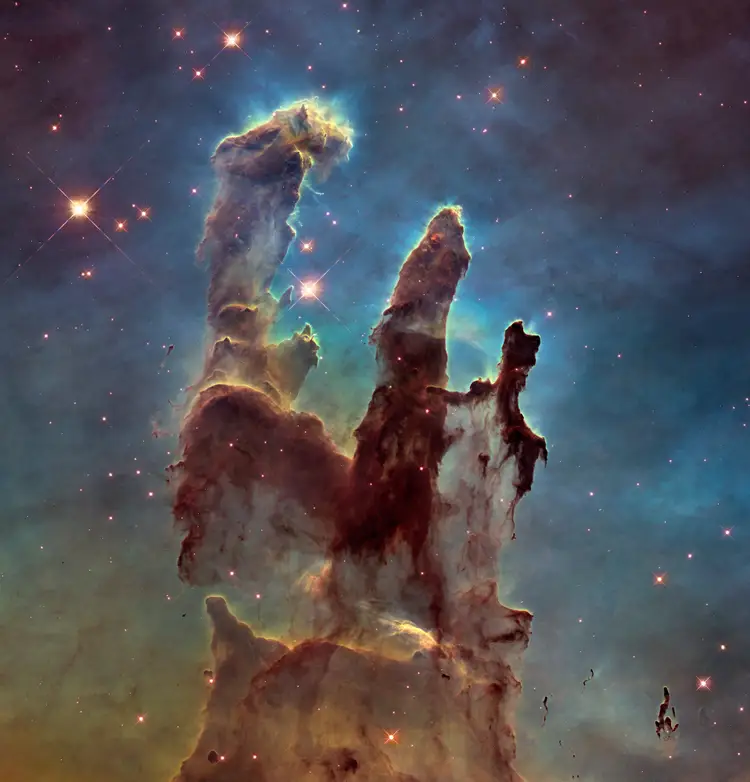
\includegraphics[width=\paperwidth]{book-cover.png}};
\draw (current page.center) node [fill=ocre!30!white,fill opacity=0.6,text opacity=1,inner sep=1cm]{\Huge\centering\bfseries\sffamily\parbox[c][][t]{\paperwidth}{\centering Code Review Guidebook\\[15pt] % Book title
{\Large A \textbf{Java} Guide}\\[20pt] % Subtitle
{\huge Jack Liu}}}; % Author name
\end{tikzpicture}
\vfill
\endgroup

%----------------------------------------------------------------------------------------
%	COPYRIGHT PAGE
%----------------------------------------------------------------------------------------

\newpage
~\vfill
\thispagestyle{empty}

\noindent Copyright \copyright\ 2019 Jiaqi Liu\\ % Copyright notice

\noindent \textsc{Published by Publisher}\\ % Publisher

\noindent \textsc{book-website.com}\\ % URL

\noindent Licensed under the Creative Commons Attribution-NonCommercial 3.0 Unported License (the ``License''). You may not use this file except in compliance with the License. You may obtain a copy of the License at \url{http://creativecommons.org/licenses/by-nc/3.0}. Unless required by applicable law or agreed to in writing, software distributed under the License is distributed on an \textsc{``as is'' basis, without warranties or conditions of any kind}, either express or implied. See the License for the specific language governing permissions and limitations under the License.\\ % License information, replace this with your own license (if any)

\noindent \textit{First printing, March 2019} % Printing/edition date

%----------------------------------------------------------------------------------------
%	TABLE OF CONTENTS
%----------------------------------------------------------------------------------------

%\usechapterimagefalse % If you don't want to include a chapter image, use this to toggle images off - it can be enabled later with \usechapterimagetrue

\chapterimage{chapter_head_1.pdf} % Table of contents heading image

\pagestyle{empty} % Disable headers and footers for the following pages

\tableofcontents % Print the table of contents itself

\cleardoublepage % Forces the first chapter to start on an odd page so it's on the right side of the book

\pagestyle{fancy} % Enable headers and footers again

%----------------------------------------------------------------------------------------
%	PART
%----------------------------------------------------------------------------------------

\part{Part One - Reviewing Code}

\chapterimage{chapter_head_2.pdf}

\chapter{Communication}

\section{Know What You Want to Say}

Probably the most difficult part of the more formal styles of code review comment used in business is working out exactly what it is you want to say.

Plan what you want to say. Write an outline. Then ask yourself, “Does this get across whatever I'm trying to say?” Refine it until it does. Jot down the ideas you want to communicate, and plan a couple of strategies for getting them across.

\section{Know the Code Author}

You're communicating only if you're conveying information(code changes). The following technique helps you to structure your code review commetns:

\begin{tcolorbox}[
    title = The \textbf{WISDOM} acrostic - understanding the audience(code author)
]

\textbf{W}hat do you want them to learn?

What is their \textbf{i}nterest in what you've got to say?

How \textbf{s}ophisticated are they?

How much \textbf{d}etail do they want?

Whom do you want to \textbf{o}wn the information?

How can you \textbf{m}otivate them to listen to you?

\end{tcolorbox}

\section{Choose a Style}

Adjust the style of your delivery to suit your audience. Some people want a formal “just the facts” briefing. Others like a long, wide-ranging chat before getting down to business. When it comes to written documents, some like to receive large bound reports, while others expect a simple memo or e-mail. If in doubt, ask.

Thinking about the other side's style is important, keeping you, one side of communication as well, clear is also important.

\section{Make It Look Good}

Your ideas are important. They deserve a good-looking vehicle to convey them to your audience.

Too many developers (i.e. code reviewers) concentrate solely on content when producing written code review comments. We think this is a mistake. Any chef will tell you that you can slave in the kitchen for hours only to ruin your efforts with poor presentation.

There is no excuse today for producing poor-looking code reviews. Modern word processors (along with layout systems such as markdown) can produce stunning output. You need to learn just a few basic rules.

Making a good-looking review encourages not only you, but also the other side to read it with enjoyable experiences.

\section{Be a Listener}

There's one technique that you must use if you want people to listen to you: listen to them. Even if this is a situation where you have all the information, even if this is a formal meeting with you standing in front of 20 suits—if you don't listen to them, they won't listen to you.

Encourage people to talk by asking questions. Turn the meeting into a dialog, and you'll make your point more effectively. Who knows, you might even learn something.


\chapterimage{chapter_head_2.pdf}

\chapter{You Are Partially Responsible for the Code}

Responsibility is something you actively agree to. You make a commitment, by reviewing code, to ensure that something is done right, but you don't necessarily
have direct control over every aspect of it. In addition to doing your own
personal best, you must analyze the situation for risks that are beyond
your control.

When you do accept the responsibility(because you are reviewing) for some codes, you should expect to be held accountable for it. When you see a mistake (as all programmers do) or an error in judgment, speak it out honestly and try to offer options for code authors.

Don't blame someone or something else, it is up to you to provide solutions.

\begin{marker}
Provide Options, Don't Make Lame Excuses
\end{marker}
\chapterimage{chapter_head_2.pdf}

\chapter{Keep Entropy in Mind while Reviewing}

\section{What is Software Entropy?}

While software development is immune from almost all physical laws, entropy hits us hard. Entropy is a term from physics that refers to the amount of “disorder” in a system. Unfortunately, the laws of thermodynamics guarantee that the entropy in the universe tends toward a maximum. When disorder increases in software, programmers call it “software rot.”

There are many factors that can contribute to software rot. The most important one seems to be the psychology, or culture, at work on a project. Even if you are a team of one, your project's psychology can be a very delicate thing. Despite the best laid plans and the best people, a project can still experience ruin and decay during its lifetime. Yet there are other projects that, despite enormous difficulties and constant setbacks, successfully fight nature's tendency toward disorder and manage to come out pretty well.

What makes the difference? The broken-window theory explains it.

\begin{marker}
Spot "Broken Windows" and ask code author to fix it right away.
\end{marker}

\chapterimage{chapter_head_2.pdf}

\chapter{Size of Pull Request}

\section{How Big is Appropriate?}

The story of Stone Soup and Boiled Frogs(https://en.wikipedia.org/wiki/Stone\_Soup) told us one thing about dealing with politics of software developments:

You may be in a situation where you know exactly what needs doing and how to do it. The entire system just appears before your eyes—you know it's right. But ask permission to tackle the whole thing and you'll be met with delays and blank stares. People will form committees, budgets will need approval, and things will get complicated. Everyone will guard their own resources. Sometimes this is called “start-up fatigue.”

It's time to bring out the stones. Work out what you can reasonably ask for. Develop it well. Once you've got it, show people, and let them marvel. Then say “of course, it would be better if we added .” Pretend it's not important. Sit back and wait for them to start asking you to add the functionality you originally wanted. People find it easier to join an ongoing success. Show them a glimpse of the future and you'll get them to rally around

Code reviewers should judge the size of a PR using SS story as a guidance, is this change small enough to start something which can be shown to people? If it's too big, as code author to break it into multiple PR's

\begin{marker}
Be a Catalyst for Change
\end{marker}

Keeping the PR size small has another advantage. Consider the other side. The villagers think about the stones and forget about the rest of the world. We all fall for it, every day. Things just creep up on us.

We've all seen the symptoms. Projects slowly and inexorably get totally out of hand. Most software disasters start out too small to notice, and most project overruns happen a day at a time. Systems drift from their specifications feature by feature, while patch after patch gets added to a piece of code until there's nothing of the original left. It's often the accumulation of small things that breaks morale and teams.

\begin{marker}
As a code reviewer, always remember the Big Picture
\end{marker}

\chapterimage{chapter_head_2.pdf}

\chapter{Avoid Duplication}

\section{DRY}

Unfortunately, knowledge isn't stable. It changes—often rapidly. Your understanding of a requirement may change following a meeting with the client. The government changes a regulation and some business logic gets outdated. Tests may show that the chosen algorithm won't work. All this instability means that we spend a large part of our time in maintenance mode, reorganizing and reexpressing the knowledge in our systems.

Most people assume that maintenance begins when an application is released, that maintenance means fixing bugs and enhancing features. We think these people are wrong. Programmers are constantly in maintenance mode. Our understanding changes day by day. New requirements arrive as we're designing or coding. Perhaps the environment changes. Whatever the reason, maintenance is not a discrete activity, but a routine part of the entire development process.

When we perform maintenance, we have to find and change the representations of things—those capsules of knowledge embedded in the application. The problem is that it's easy to duplicate knowledge in the specifications, processes, and programs that we develop, and when we do so, we invite a maintenance nightmare—one that starts well before the application ships.

We feel that the only way to develop software reliably, and to make our developments easier to understand and maintain, is to follow what we call the DRY(Don't Repeat Yourself) principle:

\begin{remark}
EVERY PIECE OF KNOWLEDGE MUST HAVE A SINGLE, UNAMBIGUOUS, AUTHORITATIVE REPRESENTATION WITHIN A SYSTEM.
\end{remark}

\begin{marker}
On duplicated codes, ask code author to remove it
\end{marker}

\section{How Does Duplication Arise?}

Most of the duplication we see falls into one of the following categories:

\begin{itemize}
    \item \textbf{Imposed duplication} Developers feel they have no choice—the environment seems to require duplication.
    \item \textbf{Inadvertent duplication}  Developers don't realize that they are duplicating information.
    \item \textbf{Impatient duplication}  Developers get lazy and duplicate because it seems easier.  
    \item \textbf{Inter-developer duplication}  Multiple people on a team (or on different
teams) duplicate a piece of information.
\end{itemize}

\chapterimage{chapter_head_2.pdf}

\chapter{Meaningful Names}

The hardest thing about choosing good names is that it requires \textbf{good descriptive skills} and \textbf{a shared cultural background}. This is a teaching issue rather than a technical, business, or management issue. As a result many people in this field don't learn to do it very well.

Follow the rules above and do not afraid to make changes on other's code accordinly. It pays in both short and long terms

\section{Use Intention-Revealing Names}\index{Naming!Use Intention-Revealing Names}

Everyone who reads your code (including you) will be happier if you take care with your naming.

\subsection{Variable Declaration should not \textit{require} a comment}

\href{https://checkstyle.sourceforge.io/config_javadoc.html?--#JavadocVariable}{While it is a good Java practice to comment variables of a class}, the name of a variable, function, or class, should have already answered all the big questions. It should tell you why it exists, what it does, and how it is used.
If a name requires a comment, then the name does not reveal its intent.

\begin{marker}
\textbf{If a name requires a comment, then the name does not reveal its intent.}
\end{marker}

For example:

\begin{tcolorbox}[breakable, colback=red!10!white, colframe=red!85!black, sidebyside, righthand width = 3cm, tikz lower]

\begin{lstlisting}[language = java]
int d; // elapsed time in days
\end{lstlisting}

\tcblower

\path[fill = yellow, draw = yellow!75!red] (0, 0) circle (1cm);
\fill[red] (45:5mm) circle (1mm);
\fill[red] (135:5mm) circle (1mm);
\draw[line width=1mm,red] (230:6mm) arc (145:35:5mm);

\end{tcolorbox}

The name \ubuntubox{\lstinline{d}} reveals nothing. It does not evoke a sense of elapsed time, nor of days. We should choose a name that specifies what is being measured and the unit of that measurement:

\begin{tcolorbox}[breakable, colback=green!10!white, colframe=green!85!black, sidebyside, righthand width = 3cm, tikz lower]

\begin{lstlisting}[language = java]
int elapsedTimeInDays;
int daysSinceCreation;
int daysSinceModification;
int fileAgeInDays;
\end{lstlisting}

\tcblower

\path[fill = yellow, draw = yellow!75!red] (0, 0) circle (1cm);
\fill[red] (45:5mm) circle (1mm);
\fill[red] (135:5mm) circle (1mm);
\draw[line width=1mm,red] (215:5mm) arc (215:325:5mm);

\end{tcolorbox}

\subsection{Promote simplicity and \textbf{IMPLICITY}}

\begin{tcolorbox}[breakable, colback=red!10!white, colframe=red!85!black, sidebyside, righthand width = 3cm, tikz lower]

\begin{lstlisting}[language = java]
public List<int[]> getThem() {
    List<int[]> list1 = new ArrayList<int[]>();
    
    for (int[] x : theList) {
        if (x[0] == 4) {
            list1.add(x);
        }
    }

    return list1;
}
\end{lstlisting}

\tcblower

\path[fill = yellow, draw = yellow!75!red] (0, 0) circle (1cm);
\fill[red] (45:5mm) circle (1mm);
\fill[red] (135:5mm) circle (1mm);
\draw[line width=1mm,red] (230:6mm) arc (145:35:5mm);

\end{tcolorbox}

Why is it hard to tell what this code is doing? Although code syntax is not complicated, the problem is not the simplicity of the code but the \textit{implicity} of the code.

\begin{definition}[Implicity of the Code]
The degree to which the context is not explicit in the code itself
\end{definition}

The code implicitly requires that we know the answers to questions such as:

\begin{itemize}
    \item What kinds of things are in \inlinecode[blue]{theList}?
    \item What is the significance of the zeroth subscript of an item in \inlinecode[blue]{theList}?
    \item What is the significance of the value 4?
    \item How would I use the list being returned?
\end{itemize}

The answers to these questions are not present in the code sample, but they could have been.

\begin{marker}
\textbf{The code review should point out the problem and the re-review should make sure that simplicity of the code has not changed.}
\end{marker}

\section{Avoid Disinformation}\index{Naming!Avoid Disinformation}

\subsubsection{Sub-type Naming}

Java usually declares variables by type and always assigns variables with concrete implementation. A variable should not be named by a sub-type name if the type could be different type nature. For example, when a variable's type is \inlinecode[blue]{Collection} and is assigned a \inlinecode[blue]{ArrayList}, it should not be named as something like \inlinecode[red]{peopleList}; instead \inlinecode[green]{peopleGroup} or simply \inlinecode[green]{persons} would be better.

\begin{marker}
\textbf{A variable should not be named by a sub-type name if the type could be different type nature.}
\end{marker}

\subsubsection{Avoid Names That Vary in Small Ways}

Long and smilarly-named variables are very hard for people to read and distinguish. For example How long does it take to spot the subtle difference between a \inlinecode[red]{XYZControllerForEfficientHandlingOfStrings} in one module and, somewhere a little more distant, \inlinecode[red]{XYZControllerForEfficientStorageOfStrings}?

In addition, developer using IDE uses auto-complete feature. They will often blindly pick up the wrong variable simply because the two looks so similar.

\section{Make Meaningful Distinctions}\index{Naming!Make Meaningful Distinctions}

By all possible means, people could name two things with non-meaningful distinctions. For example, class \inlinecode[red]{Product} v.s. class \inlinecode[red]{ProductInfo}. What are the difference between the two? Product can have product info, too. Same issues goes for methods:

\begin{tcolorbox}[breakable, colback=red!10!white, colframe=red!85!black, sidebyside, righthand width = 3cm, tikz lower]

\begin{lstlisting}[language = java]
getActiveAccount();
getActiveAccounts();
getActiveAccountInfo();
\end{lstlisting}

\tcblower

\path[fill = yellow, draw = yellow!75!red] (0, 0) circle (1cm);
\fill[red] (45:5mm) circle (1mm);
\fill[red] (135:5mm) circle (1mm);
\draw[line width=1mm,red] (230:6mm) arc (145:35:5mm);

\end{tcolorbox}

How are the programmers in this project supposed to know which of these functions to call?

\subsection{Use Speakable/Pronouncable Names}\index{Naming!Use Speakable/Pronouncable Names}

\begin{remark}
Humans are good at words. A significant part of our brains is dedicated to the concept of words. Words are pronounceable
\end{remark}

If you can't pronounce it, you can't discuss it without sounding like an idiot. “Well, over here on the bee cee arr three cee enn tee we have a pee ess zee kyew int, see?” This matters because \textit{programming is a social activity}.

\begin{marker}
Use Speakable/Pronounceable Names
\end{marker}

\section{Use Searchable Names}\index{Naming!Use Searchable Names}

Single-letter names and numeric constants have a particular problem in that they are not easy to locate across a body of text.

My personal preference is that single-letter names can ONLY be used as local variables inside short methods.\textit{The length of a name should correspond to the size of its scope} If a variable or constant might be seen or used in multiple places in a body of code, it is imperative to give it a search-friendly name.

\begin{marker}
Use Searchable Names
\end{marker}

\section{Don't Add Gratuitous Context}\index{Naming!Don't Add Gratuitous Context}

In an imaginary application called “Gas Station Deluxe,” it is a bad idea to prefix every class with \inlinecode[red]{GSD}. Frankly, you are working against your tools. You type "G" and press the completion key and are rewarded with a mile-long list of every class in the system. Is that wise? Why make it hard for the IDE to help you?

Likewise, say you invented a \inlinecode[blue]{MailingAddress} class in GSD's accounting module, and you named it \inlinecode[red]{GSDAccountAddress}. Later, you need a mailing address for your customer contact application. Do you use \inlinecode[red]{GSDAccountAddress}? Does it sound like the right name? Ten of 17 characters are redundant or irrelevant.

Shorter names are generally better than longer ones, so long as they are clear. Add no more context to a name than is necessary.

The names \inlinecode[green]{accountAddress} and \inlinecode[green]{customerAddress} are fine names for instances of the class \inlinecode[blue]{Address} but could be poor names for classes. \inlinecode[green]{Address} is a fine name for a class. If I need to differentiate between MAC addresses, port addresses, and Web addresses, I might
consider \inlinecode[green]{PostalAddress}, \inlinecode[green]{MAC}, and \inlinecode[green]{URI}. The resulting names are more precise, which is the point of all naming.
\chapterimage{chapter_head_2.pdf}

\chapter{Functions}

Every system is built from a domain-specific language designed by the programmers to describe that system. Functions are the verbs of that language, and classes are the nouns. This is a much older truth. The art of programming is, and has always been, the art of language design.

Master programmers think of systems as stories to be told rather than programs to be written. They use the facilities of their chosen programming language to construct a much richer and more expressive language that can be used to tell that story. Part of that domain-specific language is the hierarchy of functions that describe all the actions that take place within that system. In an artful act of recursion those actions are written to use the very domain-specific language they define to tell their own small part of the story.

To write functions/methods well(and, of course, reviewing other's methods), in addition to following the rules below, you need to let the author know that writing software is like any other kind of writing. When you write a paper or an article,
you get your thoughts down first, then you massage it until it reads well. The first draft might be clumsy and disorganized, so you wordsmith it and restructure it and refine it until it reads the way you want it to read.

When I write functions, they come out long and complicated. They have lots of
indenting and nested loops. They have long argument lists. The names are arbitrary, and there is duplicated code. But I also have a suite of unit tests that cover every one of those clumsy lines of code. So then I massage and refine that code, splitting out functions, changing names, eliminating duplication. I shrink the methods and reorder them. Sometimes I break out whole classes, all the while keeping the tests passing.

In the end, I wind up with functions that follow the rules I've laid down in this chapter. I don't write them that way to start. I don't think anyone could.

\begin{tcolorbox}[breakable, colback=green!10!white, colframe=green!85!black, center title, title = Golden Rule of Functions]
\begin{center}
As small as possible
\end{center}
\end{tcolorbox}

\section{Blocks and Indenting}\index{Functions! Blocks and Indenting}

The blocks within \inlinecode[green]{if} statements, \inlinecode[green]{else} statements, \inlinecode[green]{while} statements, and so on should be one line long. Probably that line should be a function call. Not only does this keep the enclosing function small, but it also adds documentary value because the
function called within the block can have a nicely descriptive name.

This also implies that functions should not be large enough to hold nested structures. Therefore, the indent level of a function should not be greater than one or two. This, of course, makes the functions easier to read and understand.

For example:

\begin{tcolorbox}[breakable, colback=red!10!white, colframe=red!85!black, sidebyside, righthand width = 3cm, tikz lower, label=blocks-and-indenting-bad]

\begin{lstlisting}[language = java, basicstyle=\small]
public static String renderPageWithSetupsAndTeardowns(
        PageData pageData,
        boolean isSuite
) throws Exception {
    boolean isTestPage = pageData.hasAttribute("Test");
    if (isTestPage) {
        WikiPage testPage = pageData.getWikiPage();
        StringBuffer newPageContent = new StringBuffer();
        includeSetupPages(testPage, newPageContent, isSuite);
        newPageContent.append(pageData.getContent());
        includeTeardownPages(testPage, newPageContent, isSuite);
        pageData.setContent(newPageContent.toString());
    }

    return pageData.getHtml();
}
\end{lstlisting}

\tcblower

\path[fill = yellow, draw = yellow!75!red] (0, 0) circle (1cm);
\fill[red] (45:5mm) circle (1mm);
\fill[red] (135:5mm) circle (1mm);
\draw[line width=1mm,red] (230:6mm) arc (145:35:5mm);

\end{tcolorbox}

\begin{tcolorbox}[breakable, colback=green!10!white, colframe=green!85!black, sidebyside, righthand width = 3cm, tikz lower, label=blocks-and-indenting-good]

\begin{lstlisting}[language = java, basicstyle=\small]
public static String renderPageWithSetupsAndTeardowns(
        PageData pageData,
        boolean isSuite
) throws Exception {
    if (isTestPage(pageData)) {
        includeSetupAndTeardownPages(
                pageData,
                isSuite
        );
    }
    return pageData.getHtml();
}
\end{lstlisting}

\tcblower

\path[fill = yellow, draw = yellow!75!red] (0, 0) circle (1cm);
\fill[red] (45:5mm) circle (1mm);
\fill[red] (135:5mm) circle (1mm);
\draw[line width=1mm,red] (215:5mm) arc (215:325:5mm);

\end{tcolorbox}

\begin{marker}
The blocks within \inlinecode[green]{if} statements, \inlinecode[green]{else} statements, \inlinecode[green]{while} statements, and so on should be one line long.
The indent level of a function should not be greater than one or two.
\end{marker}

\section{Do One Thing}\index{Functions!Do One Thing}

While everybody understands the following rule:

\begin{tcolorbox}[breakable, colback=green!10!white, colframe=green!85!black, center title]
\begin{center}
FUNCTIONS SHOULD DO ONE THING. THEY SHOULD DO IT WELL.
THEY SHOULD DO IT ONLY.
\end{center}
\end{tcolorbox}

the problem with this statement is that it is hard to know what “one thing” is. Does Listing~\ref{blocks-and-indenting-good} do one thing? It's easy to make the case that it's doing three things:

\begin{enumerate}
    \item Determining whether the page is a test page.
    \item If so, including setups and teardowns.
    \item Rendering the page in HTML.
\end{enumerate}

Notice that the three steps of the function are one level of abstraction below the stated name of the function. We can describe the function by describing it in JavaDoc of this method:

\begin{lstlisting}
"we check to see whether the page is a test page and if so, we include the setups and teardowns. In either case we render the page in HTML."
\end{lstlisting}

If a function does only those steps that are one level below the stated name of the function, then the function is doing one thing. After all, the reason we write functions is to decompose a larger concept (in other words, the name of the function) into a set of steps at the next level of abstraction.

Listing~\ref{blocks-and-indenting-bad} has two levels of abstraction, as proved by our ability to shrink it down. But it would be very hard to meaningfully shrink Listing~\ref{blocks-and-indenting-good}. We could extract the if statement into a function named \inlinecode[green]{includeSetupsAndTeardownsIfTestPage}, but that simply restates the code without changing the level of abstraction.

\subsection{One Level of Abstraction per Function}

In order to make sure our functions are doing “one thing,” we need to make sure that the statements within our function are all at the same level of abstraction.

It is easy to see how a mixing of \inlinecode[yellow]{getHtml()} (very high level abstraction) and \inlinecode[yellow]{string.append("\n")} (very low level abstraction) is violating this rule.

Mixing levels of abstraction within a function is always confusing. Readers may not be able to tell whether a particular expression is an essential concept or a detail. Worse, like broken windows, once details are mixed with essential concepts, more and more details tend to accrete within the function.

\begin{marker}
Do NOT mix level of abstraction in a method
\end{marker}

\section{Reading Code from Top to Bottom: The Stepdown Rule}\index{Functions!Reading Code from Top to Bottom: The Stepdown Rule}

We want the code to read like a top-down narrative.5 We want every function to be followed by those at the next level of abstraction so that we can read the program, descending one level of abstraction at a time as we read down the list of functions.

\begin{marker}
\textbf{The Stepdown Rule} - We want the code to read like a top-down narrative.5 We want every function to be followed by those at the next level of abstraction so that we can read the program, descending one level of abstraction at a time as we read down the list of functions.
\end{marker}

It turns out to be very difficult for programmers to learn to follow this rule and write functions that stay at a single level of abstraction. But learning this trick is also very important. It is the key to keeping functions short and making sure they do "one thing".

\section{Switch Statements}\index{Functions!Switch Statements}

It's hard to make a small \inlinecode[red]{switch} statement(or an equivalent if-else chains). It's also hard to make a switch statement
that does one thing. By their nature, switch statements always do N things. Unfortunately we can't always avoid switch statements, but we can make sure that each \inlinecode[red]{switch} statement is buried in a low-level class and is never repeated. We do this, of course, with
\textbf{polymorphism}.

Consider Listing~\ref{switch-statements-bad}. It shows just one of the operations that might depend on the
type of employee.

\begin{tcolorbox}[breakable, colback=red!10!white, colframe=red!85!black, sidebyside, righthand width = 3cm, tikz lower, label=switch-statements-bad]

\begin{lstlisting}[language = java, basicstyle=\small]
public Money calculatePay(Employee e) {
    switch (e.type) {
        case COMMISSIONED:
            return calculateCommissionedPay(e);
        case HOURLY:
            return calculateHourlyPay(e);
        case SALARIED:
            return calculateSalariedPay(e);
        default:
            // exception
    }
}
\end{lstlisting}

\tcblower

\path[fill = yellow, draw = yellow!75!red] (0, 0) circle (1cm);
\fill[red] (45:5mm) circle (1mm);
\fill[red] (135:5mm) circle (1mm);
\draw[line width=1mm,red] (230:6mm) arc (145:35:5mm);

\end{tcolorbox}

There are several problems with this function:

\begin{enumerate}
    \item it's large, and when new employee types are added, it will grow
    \item it very clearly does more than one thing
    \item it violates the Single Responsibility Principle because there is more than one reason for it to change
    \item it violates the Open Closed Principle because it must change whenever new types are added
    \item \textbf{WORST} - there are an unlimited number of other functions that will have the same structure. For example we could have \inlinecode[blue]{isPayday(Employee e),} or \inlinecode[blue]{deliverPay(Employee e)} or a host of others. All of which would have the same deleterious structure.
\end{enumerate}

The solution to this problem (see Listing~\ref{switch-statements-good}) is to bury the switch statement in the basement of an ABSTRACT FACTORY and never let anyone see it. The factory will use the
switch statement to create appropriate instances of the derivatives of Employee, and the various functions, such as calculatePay, isPayday, and deliverPay, will be dispatched polymorphically through the Employee interface.

\begin{tcolorbox}[breakable, colback=green!10!white, colframe=green!85!black, sidebyside, righthand width = 3cm, tikz lower, label=switch-statements-good]

\begin{lstlisting}[language = java, basicstyle=\small]
public abstract class Employee {
    public abstract boolean isPayday();
    public abstract Money calculatePay();
    public abstract void deliverPay(Money pay);
}
-----------------
public interface EmployeeFactory {
    public Employee makeEmployee(EmployeeRecord r);
}
-----------------
public class EmployeeFactoryImpl implements EmployeeFactory {

    @Override
    public Employee makeEmployee(EmployeeRecord r) {
        switch (r.type) {
            case COMMISSIONED:
                return new CommissionedEmployee(r) ;
            case HOURLY:
                return new HourlyEmployee(r);
            case SALARIED:
                return new SalariedEmploye(r);
            default:
                // exception
        }
    }
}
\end{lstlisting}

\tcblower

\path[fill = yellow, draw = yellow!75!red] (0, 0) circle (1cm);
\fill[red] (45:5mm) circle (1mm);
\fill[red] (135:5mm) circle (1mm);
\draw[line width=1mm,red] (215:5mm) arc (215:325:5mm);

\end{tcolorbox}

\begin{marker}
Bury the switch statement in the basement of an ABSTRACT FACTORY and never let anyone see it
\end{marker}

The general rule for \inlinecode[yellow]{switch} statements is that they can be tolerated if they

\begin{enumerate}
    \item appear only once
    \item are used to create polymorphic objects
    \item are hidden behind an inheritance relationship so that the rest of the system cannot see them
\end{enumerate}

\begin{marker}
Reduce switch(or if-else chain) statements as much as possible
\end{marker}

\section{Function Arguments}\index{Functions!Function Arguments}

The ideal number of arguments for a function is zero (niladic). Next comes one (monadic), followed closely by two (dyadic). Three arguments (triadic) should be avoided where possible. More than three (polyadic) requires very special justification—and then shouldn't be used anyway

Arguments are hard. They take a lot of conceptual power. Readers
would have had to interpret it each time they saw it. When you are reading the story told by the module, \inlinecode[green]{includeSetupPage()} is easier to understand than \inlinecode[red]{includeSetupPageInto(newPageContent)}. \textbf{The argument is at a different level of abstraction than the function name} and forces you to know a detail that isn't particularly important at that point.

\begin{remark}
Arguments are hard. They take a lot of conceptual power.
\end{remark}

Arguments are also hard from a testing point of view.

Output arguments are harder to understand than input arguments. When we read a function, we are used to the idea of information going in to the function through arguments and out through the return value. We don't usually expect information to be going out through the arguments. So output arguments often cause us to do a double-take.

\begin{marker}
Reduce the number of arguments as much as possible.

No output argument
\end{marker}

\subsection{Common Monadic Forms}

There are two very common reasons to pass a single argument into a function:

\begin{enumerate}
    \item Asking a question about that argument, as in \inlinecode[green]{boolean fileExists(“MyFile”).}
    \item Operating and transforming it into something else and returning it. For example, transform a file name into content - \inlinecode[green]{InputStream fileOpen(“MyFile”)}
\end{enumerate}

These two uses are what readers expect when they see a function. You should choose names that make the distinction clear, and always use the two forms in a consistent context.

A somewhat less common, but still very useful form for a single argument function, is an \textit{event}. In this form there is an input argument but no output argument. The overall program is meant to interpret the function call as an event and use the argument to alter the state of the system.

\begin{marker}
Use monadic argument appropriately
\end{marker}

Try to avoid any monadic functions that don't follow these forms. Using an output argument instead of a return value for a transformation is confusing. If a function is going to transform its input argument, the transformation should appear as the return value.

\begin{marker}
Put output argument as return vlaue
\end{marker}

\subsection{Flag Arguments}

Flag arguments are ugly. Passing a boolean into a function is a truly terrible practice. It immediately complicates the signature of the method, loudly proclaiming that this function does more than one thing. It does one thing if the flag is true and another if the flag is false!

\begin{marker}
Split the method into 2 sub-calls to enhance readability 
\end{marker}

\subsection{Dyadic Functions}

There are times, of course, where two arguments are appropriate. For example, it is perfectly reasonable to have \inlinecode[green]{Point p = new Point(0,0);}. Cartesian points naturally take two arguments. However, the two arguments in this case are \textit{ordered components of a single value}! Whereas output-Stream and name, as in \inlinecode[red]{writeField(output-Stream, name)}, have neither a natural cohesion, nor a natural ordering.

Even obvious dyadic functions like \inlinecode[red]{assertEquals(expected, actual)} are problematic.
How many times have you put the \inlinecode[red]{actual} where the \inlinecode[red]{expected} should be? The two arguments have no natural ordering. The expected, actual ordering is a convention that requires practice to learn. This is one of the reasons I do not use junit for testing.

Dyads aren't evil, and you will certainly have to write them. However, you should be aware that they come at a cost and should take advantage of what mechanims may be available to you to convert them into monads. For example, you might make the \inlinecode[green]{writeField} method a member of \inlinecode[green]{outputStream} so that you can say \inlinecode[green]{outputStream. writeField(name)}. Or you might make the \inlinecode[green]{outputStream} a member variable of the current class so that you don't have to pass it. Or you might extract a new class like \inlinecode[green]{FieldWriter} that takes the \inlinecode[green]{outputStream} in its constructor and has a write method.

\begin{marker}
Design natural-ordering or natural-cohesion bi-arguments
\end{marker}

\section{Argument Objects}\index{Functions!Argument Objects}

When a function seems to need more than two or three arguments, it is likely that some of those arguments ought to be wrapped into a class of their own.

Consider, for example, the difference between the two following declarations:

\begin{tcolorbox}[breakable, colback=green!10!white, colframe=green!85!black, center title, sidebyside]

\begin{lstlisting}[language = java, basicstyle=\small]
Circle makeCircle(double x, double y, double radius);
\end{lstlisting}

\tcblower

\begin{lstlisting}[language = java, basicstyle=\small]
Circle makeCircle(Point center, double radius);
\end{lstlisting}

\end{tcolorbox}

Reducing the number of arguments by creating objects out of them may seem like cheating, but it's not. When groups of variables are passed together, the way x and y are in the example above, they are likely part of a concept that deserves a name of its own.

\section{Argument Lists}\index{Functions!Argument Lists}

Sometimes we want to pass a variable number of arguments into a function. Consider, for example:

\begin{tcolorbox}[breakable, colback=green!10!white, colframe=green!85!black]
\begin{lstlisting}[language = java, basicstyle=\small]
String.format("%s worked %.2f hours.", name, hours);
\end{lstlisting}
\end{tcolorbox}

If the variable arguments are all treated identically, as they are in the example above, then they are equivalent to a single argument of type List. By that reasoning, this method is actually dyadic. Indeed, the declaration of String.format as shown below is clearly dyadic:

\begin{tcolorbox}[breakable, colback=green!10!white, colframe=green!85!black]
\begin{lstlisting}[language = java, basicstyle=\small]
public String format(String format, Object... args)
\end{lstlisting}
\end{tcolorbox}

So all the same rules apply. Functions that take variable arguments can be monads, dyads, or even triads. But it would be a mistake to give them more arguments than that.

\begin{tcolorbox}[breakable, colback=green!10!white, colframe=green!85!black, sidebyside, righthand width = 3cm, tikz lower]

\begin{lstlisting}[language = java, basicstyle=\small]
void monad(Integer... args);
void dyad(String name, Integer... args);
void triad(String name, int count, Integer... args);
\end{lstlisting}

\tcblower

\path[fill = yellow, draw = yellow!75!red] (0, 0) circle (1cm);
\fill[red] (45:5mm) circle (1mm);
\fill[red] (135:5mm) circle (1mm);
\draw[line width=1mm,red] (215:5mm) arc (215:325:5mm);

\end{tcolorbox}

\section{Coherent method name and arguments}\index{Functions!Coherent method name and arguments}

Choosing good names for a function can go a long way toward explaining the intent of the function and the order and intent of the arguments. In the case of a monad, the function and argument should form a very nice verb/noun pair. For example, \inlinecode[green]{write(name)} is very evocative. Whatever this “name” thing is, it is being “written.”

\section{Have No Side Effects}\index{Functions!Have No Side Effects}

\subsection{What is Side Effects}

Side effects are lies. Your function promises to do one thing, but it also does other hidden things. Sometimes it will make unexpected changes to the variables of its own class. Sometimes it will make them to the parameters passed into the function or to system globals. In either case they are devious and damaging mistruths that often result in strange temporal couplings and order dependencies.

\subsection{Example}

\begin{tcolorbox}[breakable, colback=red!10!white, colframe=red!85!black, sidebyside, righthand width = 3cm, tikz lower]

\begin{lstlisting}[language = java, basicstyle=\small]
public class UserValidator {
    
    private Cryptographer cryptographer;

    public boolean checkPassword(String userName, String password) {
        User user = UserGateway.findByName(userName);
        if (user != User.NULL) {
            String codedPhrase = user.getPhraseEncodedByPassword();
            String phrase = cryptographer.decrypt(codedPhrase, password);
            if ("Valid Password".equals(phrase)) {
                Session.initialize();
                return true;
            }
        }
        return false;
    }
}
\end{lstlisting}

\tcblower

\path[fill = yellow, draw = yellow!75!red] (0, 0) circle (1cm);
\fill[red] (45:5mm) circle (1mm);
\fill[red] (135:5mm) circle (1mm);
\draw[line width=1mm,red] (230:6mm) arc (145:35:5mm);

\end{tcolorbox}

The side effect is the call to \inlinecode[red]{Session.initialize()}, of course. The \inlinecode[red]{checkPassword} function, by its name, says that it checks the password. The name does not imply that it initializes the session. So a caller who believes what the name of the function says runs the risk of erasing the existing session data when he or she decides to check the validity of the user.

This side effect creates a temporal coupling. That is, \inlinecode[red]{checkPassword} can only be called at certain times (in other words, when it is safe to initialize the session). If it is called out of order, session data may be inadvertently lost. Temporal couplings are confusing, especially when hidden as a side effect. If you must have a temporal coupling, you should make it clear in the name of the function. In this case we might rename the function \inlinecode[red]{checkPasswordAndInitializeSession}, though that certainly violates "Do one thing."

\begin{marker}
Watch out for side effects in review - does the method do more than what method name implies?
\end{marker}

\subsection{Output Arguments}

Output argument makes it hard to read. For example:

\begin{tcolorbox}[breakable, colback=red!10!white, colframe=red!85!black]
appendFooter(s);
\end{tcolorbox}

Does this function append s as the footer to something? Or does it append some footer to s? Is s an input or an output? It doesn't take long to look at the function signature and see:

\begin{tcolorbox}[breakable, colback=red!10!white, colframe=red!85!black]
public void appendFooter(StringBuffer report)
\end{tcolorbox}

This clarifies the issue, but only at the expense of checking the declaration of the function. Anything that forces you to check the function signature is equivalent to a double-take. It's a cognitive break and should be avoided.

\begin{marker}
Anything that forces you to check the function signature is equivalent to a double-take which should be avoided
\end{marker}

In general output arguments should be avoided. If your function must change the state of something, \textit{have it change the state of its owning objec}

\section{Command Query Separation}\index{Functions!Command Query Separation}

Functions should either do something or answer something, but not both. Either your
function should change the state of an object, or it should return some information about that object. Doing both often leads to confusion. Consider, for example, the following function:

\begin{tcolorbox}[breakable, colback=red!10!white, colframe=red!85!black, sidebyside, righthand width = 3cm, tikz lower]
\begin{lstlisting}[language = java, basicstyle=\small]
public boolean set(String attribute, String value);
\end{lstlisting}

\tcblower

\path[fill = yellow, draw = yellow!75!red] (0, 0) circle (1cm);
\fill[red] (45:5mm) circle (1mm);
\fill[red] (135:5mm) circle (1mm);
\draw[line width=1mm,red] (230:6mm) arc (145:35:5mm);
\end{tcolorbox}

This function sets the value of a named attribute and returns true if it is successful and false if no such attribute exists. This leads to odd statements like this:

\begin{tcolorbox}[breakable, colback=red!10!white, colframe=red!85!black, sidebyside, righthand width = 3cm, tikz lower]
\begin{lstlisting}[language = java, basicstyle=\small]
if (set("username", "unclebob"))...
\end{lstlisting}

\tcblower

\path[fill = yellow, draw = yellow!75!red] (0, 0) circle (1cm);
\fill[red] (45:5mm) circle (1mm);
\fill[red] (135:5mm) circle (1mm);
\draw[line width=1mm,red] (230:6mm) arc (145:35:5mm);
\end{tcolorbox}

What does it mean? It is hard to answer without reading the source code of the method(or its doc). The real solution is to separate the command from the query so that the ambiguity cannot occur:

\begin{tcolorbox}[breakable, colback=green!10!white, colframe=green!85!black, sidebyside, righthand width = 3cm, tikz lower]

\begin{lstlisting}[language = java, basicstyle=\small]
if (attributeExists("username")) {
    setAttribute("username", "unclebob");
    ...
}
\end{lstlisting}

\tcblower

\path[fill = yellow, draw = yellow!75!red] (0, 0) circle (1cm);
\fill[red] (45:5mm) circle (1mm);
\fill[red] (135:5mm) circle (1mm);
\draw[line width=1mm,red] (215:5mm) arc (215:325:5mm);

\end{tcolorbox}

\section{Prefer Exceptions to Returning Error Codes}\index{Functions~Prefer Exceptions to Returning Error Codes}

Returning error codes from command functions is a subtle violation of command query
separation:

\begin{tcolorbox}[breakable, colback=red!10!white, colframe=red!85!black, sidebyside, righthand width = 3cm, tikz lower, label=exception-over-err-code-bad]
\begin{lstlisting}[language = java, basicstyle=\small]
if (deletePage(page) == E_OK) {
    if (registry.deleteReference(page.name) == E_OK) {
        if (configKeys.deleteKey(page.name.makeKey()) == E_OK){
            logger.log("page deleted");
        } else {
            logger.log("configKey not deleted");
        }
    } else {
        logger.log("deleteReference from registry failed");
    }
} else {
    logger.log("delete failed");
    return E_ERROR;
}
\end{lstlisting}

\tcblower

\path[fill = yellow, draw = yellow!75!red] (0, 0) circle (1cm);
\fill[red] (45:5mm) circle (1mm);
\fill[red] (135:5mm) circle (1mm);
\draw[line width=1mm,red] (230:6mm) arc (145:35:5mm);
\end{tcolorbox}

Note the first line in Listing~\ref{exception-over-err-code-bad}. When you return an error code, you create the problem that the caller must \textit{deal with the error immediately}.

On the other hand, if you use exceptions instead of returned error codes, then the error processing code can be separated from the happy path code and can be simplified:

\begin{tcolorbox}[breakable, colback=green!10!white, colframe=green!85!black, sidebyside, righthand width = 3cm, tikz lower]

\begin{lstlisting}[language = java, basicstyle=\small]
try {
    deletePage(page);
    registry.deleteReference(page.name);
    configKeys.deleteKey(page.name.makeKey());
} catch (Exception e) {
    logger.log(e.getMessage());
}
\end{lstlisting}

\tcblower

\path[fill = yellow, draw = yellow!75!red] (0, 0) circle (1cm);
\fill[red] (45:5mm) circle (1mm);
\fill[red] (135:5mm) circle (1mm);
\draw[line width=1mm,red] (215:5mm) arc (215:325:5mm);

\end{tcolorbox}

Another advantage of using Exceptions is that returning error codes usually implies that there is some class or enum in which all the error codes are defined.

\begin{tcolorbox}[breakable, colback=red!10!white, colframe=red!85!black, sidebyside, righthand width = 3cm, tikz lower, label=exception-over-err-code-bad]
\begin{lstlisting}[language = java, basicstyle=\small]
public enum Error {
    OK,
    INVALID,
    NO_SUCH,
    LOCKED,
    OUT_OF_RESOURCES,
    WAITING_FOR_EVENT;
}
\end{lstlisting}

\tcblower

\path[fill = yellow, draw = yellow!75!red] (0, 0) circle (1cm);
\fill[red] (45:5mm) circle (1mm);
\fill[red] (135:5mm) circle (1mm);
\draw[line width=1mm,red] (230:6mm) arc (145:35:5mm);
\end{tcolorbox}

Classes like this are a dependency magnet; many other classes must import and use
them. Thus, when the Error enum changes, all those other classes need to be recompiled and redeployed.11 This puts a negative pressure on the Error class. Programmers don't want to add new errors because then they have to rebuild and redeploy everything. So they reuse old error codes instead of adding new ones.

When you use exceptions rather than error codes, then new exceptions are derivatives of the exception class. They can be added without forcing any recompilation or redeployment

\begin{marker}
Exception-handling, instead of Error Code, reduces coupling
\end{marker}

\section{Extract Try/Catch Blocks}\index{Functions!Extract Try/Catch Blocks}

Try/catch blocks are ugly in their own right. They confuse the structure of the code and mix error processing with normal processing. So it is better to extract the bodies of the try and catch blocks out into functions of their own.

Functions should do one thing. Error handing is one thing. Thus, a function that handles errors should do nothing else. This implies (as in the example above) that if the keyword try exists in a function, it should be the very first word in the function and that there should be nothing after the catch/finally blocks.

\begin{marker}
Put try-catch in a method and nothing else
\end{marker}

\chapterimage{chapter_head_2.pdf}

\chapter{Constructors}

\section{Constructors in general}

A  conventional distinction is made in Java between the "default constructor" and a "no-argument constructor":

\begin{definition}[Default constructor]
The default constructor\index{Constructors!default constructor} is the constructor provided by the system in the absence of any constructor provided by the programmer. Once a programmer supplies any constructor whatsoever, the default constructor is no longer supplied.
\end{definition}

\begin{definition}[No-args constructor]
A no-argument constructor\index{Constructors!no-argument constructor}, on the other hand, is a constructor provided by the programmer which takes no arguments. This distinction is necessary because the behavior of the two kinds of constructor are unrelated: a default constructor has a fixed behavior defined by Java, while the behavior of a no-argument constructor is defined by the application programmer.
\end{definition}

\begin{marker}
    It is important that JavaDoc comments makes clear distinctions between the two types of constructors. Watch out for any discrepancies in author's code.
\end{marker}

\section{Do Not Pass 'this' out of a Constructor}\index{Constructors!Do Not Pass 'this' out of a Constructor}

Within a class, the \mintinline{java}{this} Java keyword refers to the native object, the current instance of the class. Within a constructor, you can use the keyword in 3 different ways:

\begin{itemize}
    \item on the first line, you can call another constructor, using \mintinline{java}{this(...);}
    \item as a qualifier when referencing fields, as in \mintinline{java}{this.name;}
    \item as a reference passed to a method of some other object, as in \mintinline{java}{blah.operation(this);}
\end{itemize}

You can get into trouble with the last form. The problem is that, inside a constructor, the object is not yet fully constructed.

\begin{remark}
    An object is only fully constructed after its constructor completely returns, and not before
\end{remark}

But when passed as a parameter to a method of some other object, the this reference should always refer to a fully-formed object. This problem occurs mainly with listeners. Here's an example which illustrates the point:

\begin{minted}{java}
import java.util.Observable;
import java.util.Observer;

public final class EscapingThisReference {

    // A RadioStation is observed by the people listening to it.
    static final class RadioStation extends Observable {
        // elided
    }

    /*
    * A listener which waits until this object is fully-formed before it lets it be referenced by the outside world.
    * Uses a private constructor to first build the object, and then configures the fully-formed object as a listener.
    */
    static final class GoodListener implements Observer {

        /** Factory method. */
        static GoodListener buildListener(String personsName, RadioStation station) {
            //first call the private constructor
            GoodListener result = new GoodListener(personsName);
            //the 'result' object is now fully constructed, and can now be
            //passed safely to the outside world
            station.addObserver(result);
            return result;
        }

        @Override
        public void update(Observable station, Object data) {
            //..elided
        }

        private String personsName;

        /** Private constructor. */
        private GoodListener(String personsName) {
            this.personsName = personsName; //ok
        }
    }
    /**
    * A listener which incorrectly passes a 'this' reference to the outside world before construction is completed.
    */
    static final class BadListenerExplicit implements Observer {

        /** Ordinary constructor. */
        BadListenerExplicit(String personsName, RadioStation station) {
            this.personsName = personsName; //OK
            //DANGEROUS - the 'this' reference shouldn't be passed to the listener,
            //since the constructor hasn't yet completed; it doesn't matter if
            //this is the last statement in the constructor!
            station.addObserver(this);
        }

        @Override
        public void update(Observable station, Object data) {
        //..elided
        }

        private String personsName;
    }
    /**
    * Another listener that passes out a 'this' reference to the outside  world before construction is completed; here,
    * the 'this' reference is implicit, via the anonymous inner class.
    */
    static final class BadListenerImplicit {

        /** Ordinary constructor. */
        BadListenerImplicit(String personsName, RadioStation station) {
            this.personsName = personsName; //OK
            //DANGEROUS
            station.addObserver(
                new Observer() {
                    @Override
                    public void update(Observable observable, Object data) {
                        doSomethingUseful();
                    }
                });
        }

        private void doSomethingUseful() {
            //..elided
        }

        private String personsName;
    }
}
\end{minted}

\begin{marker}
    Find and tell code authors to avoid passing \mintinline{java}{this} out of constructor 
\end{marker}

\section{Avoid JavaBeans Style of Construction}\index{Constructors!Avoid JavaBeans Style of Construction}

Constructing a Model Object in many steps, first by calling a no-argument constructor, and then by calling a series of setXXX methods, is something to be avoided, if possible, because:

\begin{itemize}
    \item it is more complex, since one call is replaced with many
    \item there is no simple way to ensure that all necessary setXXX methods are called
    \item there is no simple way to implement a class invariant
    \item it allows the object to be in intermediate states which are not immediately useful, and perhaps even invalid
    \item it is not compatible with the (very useful) immutable object pattern
    \item it does not follow the style of many design patterns, in which concrete classes usually have arguments passed to their constructor. This is a recurring theme in the Design Patterns book. Constructors usually act as a "back door" for data which is needed by an implementation, but which cannot appear in the signature of some higher-level abstraction (since it would pollute such an abstraction with data specific to an implementation)
\end{itemize}

Of course, JavaBeans follow this pattern of "no-argument constructor plus setXXX". However, JavaBeans were originally intended for a very narrow problem domain - manipulation of graphical components in an IDE. As a model for the construction of typical data-centric objects (Model Objects), JavaBeans seem completely inappropriate. One can even argue strongly that, for Model Objects, the JavaBeans style is an anti-pattern, and should be avoided unless absolutely necessary.

Reading \href{https://www.oracle.com/technetwork/java/javase/documentation/spec-136004.html}{JavaBeans Spec} helps you completely understand why JavaBean is not a good idea in this context. It is important to understand Java Beans in terms of how Java is used today. The bean initiates itself as a GUI concept. Java today refers to "bean" in a completely different context defined by its popularities in non-GUI developments.

\begin{definition}{What is a Bean (Historically)?}
A Java Bean is a reusable software component that can be manipulated visually in a builder tool.
\end{definition}

Simply put, this is defined in the old Java Applet in which you click through to configure the applet before you hit run. The bean is used to record what you clicked and later spins up the program accordingly.

But today you do not hear Java Applet anymore, but you still hear about beans. Why? Because bean is usable to other popular contexts. One of them is JPA (or Persistent Storage)

This is very clear and simple. No mention is made here, or anywhere else in the specification, of Model Objects used to encapsulate database records. The whole idea of a Model Object is entirely absent from the Java Bean specification, and for good reason: the manipulation of graphical controls and the representation of database records(See 2.1.1 Beans v. Class Libraries in \href{https://www.oracle.com/technetwork/java/javase/documentation/spec-136004.html}{JavaBeans Spec}) are unrelated issues.

The life cycle of a Java Bean, starting with its no-argument constructor, is derived mainly from the task of configuring a graphical control having some default initial state. For the intended domain, this is indeed a reasonable design. For Model Objects, however, the idea of configuration in this sense is entirely meaningless.

The role of a Model Object is to carry data. Since a no-argument constructor can only build an object that is initially empty, then it cannot contribute directly to this aim. It does not form a natural candidate for the design of a Model Object.

To put data into empty Java Beans, frameworks typically call various setXXX methods using reflection. There is nothing to prevent them from calling constructors in exactly the same way.

The widespread adoption of Java Beans as a supposedly appropriate design for Model Objects seems to be an error.

\begin{marker}
    Unless absolutely necessary, do not set through objects.
\end{marker}

\section{Initializing fields to 0, false, or null is redundant}\index{Constructors!Initializing fields to 0, false, or null is redundant}

One of the most fundamental aspects of a programming language is how it initializes data. For Java, this is defined explicitly in the language specification(\lstinline{https://docs.oracle.com/javase/specs/jls/se8/html/jls-4.html#jls-4.12.5}). For fields and array components, when items are created, they are automatically set to the following default values by the system:

\begin{itemize}
    \item numbers: 0 or 0.0
    \item booleans: false
    \item object references: null
\end{itemize}

This means that explicitly setting fields to 0, false, or null (as the case may be) is unnecessary and redundant. Since this language feature was included in order to, in part, reduce repetitive coding, it's a good idea to take full advantage of it. Insisting that fields should be explicitly initialized to 0, false, or null is an idiom which is likely inappropriate to the Java programming language

Furthermore, setting a field explicitly to 0, false, or null may even cause the same operation to be performed twice (depending on your compiler). For example:

\begin{minted}{java}
public final class Quark {

    public Quark(String aName, double aMass){
        fName = aName;
        fMass = aMass;
    }

    //PRIVATE

    //WITHOUT redundant initialization to default values
    //private String fName;
    //private double fMass;

    //WITH redundant initialization to default values
    private String fName = null;
    private double fMass = 0.0d;
}
\end{minted}

If the bytecode of the Quark class is examined, the duplicated operations become clear (here, Oracle's javac compiler was used):


\begin{tcolorbox}[
skin=bicolor,colframe=blue!70!black,fonttitle=\bfseries,
    colback=blue!20!white,colbacklower=green!20!white,left=0ex,right=0ex,
    sidebyside,
  title={Title in the first language},
  after title={\hfill Title in the second language},
  width=\linewidth*1
  ]
    \begin{lstlisting}
    >javap -c -classpath . Quark
Compiled from Quark.java
public final class Quark extends java.lang.Object {
public Quark(java.lang.String,double);
}

Method Quark(java.lang.String,double)
0 aload_0
1 invokespecial #1 <Method java.lang.Object()>
4 aload_0
5 aload_1
6 putfield #2 <Field java.lang.String fName>
9 aload_0
10 dload_2
11 putfield #3 <Field double fMass>
14 return
    \end{lstlisting}
    \tcblower

    \begin{lstlisting}
    >javap -c -classpath . Quark
Compiled from Quark.java
public final class Quark extends java.lang.Object {
public Quark(java.lang.String,double);
}

Method Quark(java.lang.String,double)
0 aload_0
1 invokespecial #1 <Method java.lang.Object()>
4 aload_0
5 aconst_null
6 putfield #2 <Field java.lang.String fName>
9 aload_0
10 dconst_0
11 putfield #3 <Field double fMass>
14 aload_0
15 aload_1
16 putfield #2 <Field java.lang.String fName>
19 aload_0
20 dload_2
21 putfield #3 <Field double fMass>
24 return
    \end{lstlisting}
\end{tcolorbox}

\section{Constructors Shouldn't Start Threads}\index{Constructors!Constructors Shouldn't Start Threads}

There are two problems with starting a thread in a constructor (or static initializer):

\begin{enumerate}
    \item in a non-final class, it increases the danger of problems with subclasses
    \item it opens the door for allowing the this reference to be passed to another object before the object is fully constructed
\end{enumerate}
    

There's nothing wrong with creating a thread object in a constructor or static initializer - just don't start it there.
\chapterimage{chapter_head_2.pdf}

\chapter{Comments}

\section{Comments Do Not Make Up for Bad Code}\index{Comments!Comments Do Not Make Up for Bad Code}

One of the more common motivations for writing comments is bad code. We write a module
and we know it is confusing and disorganized. We know it's a mess. So we say to ourselves,
“Ooh, I'd better comment that!” No! You'd better clean it!
Clear and expressive code with few comments is far superior to cluttered and complex
code with lots of comments. Rather than spend your time writing the comments that
explain the mess you've made, spend it cleaning that mess.

\section{Explain Yourself as Code}\index{Comments!Explain Yourself in Code}

There are certainly times when code makes a poor vehicle for explanation. Unfortunately, many programmers have taken this to mean that code is seldom, if ever, a good means for explanation. This is patently false. Which would you rather see? This:

\begin{tcolorbox}[breakable, colback=blue!10!white, colframe=blue!85!black]

\begin{lstlisting}[language = java, basicstyle=\small]
// Check to see if the employee is eligible for full benefits
if ((employee.flags & HOURLY_FLAG) && (employee.age > 65))
\end{lstlisting}

\tcblower

\begin{lstlisting}[language = java, basicstyle=\small]
if (employee.isEligibleForFullBenefits())
\end{lstlisting}

\end{tcolorbox}

It takes only a few seconds of thought to explain most of your intent in code. In many cases it's simply a matter of creating a function that says the same thing as the comment you want to write.

\begin{marker}
If there is a comment for a piece of logic, it might be a sign of review comments saying "this should be turned into a method"
\end{marker}

\section{Good Comments}\index{Comments!Good Comments}

Some comments are necessary or beneficial. The only truly good comment is the comment you found a way not to write.

\subsection{Legal Comments}

\begin{tcolorbox}[breakable, colback=green!10!white, colframe=green!85!black, title = An Example]

\begin{verbatim}
/*
 * Copyright <some author>
 *
 * Licensed under the Apache License, Version 2.0 (the "License");
 * you may not use this file except in compliance with the License.
 * You may obtain a copy of the License at
 *
 *     http://www.apache.org/licenses/LICENSE-2.0
 *
 * Unless required by applicable law or agreed to in writing, software
 * distributed under the License is distributed on an "AS IS" BASIS,
 * WITHOUT WARRANTIES OR CONDITIONS OF ANY KIND, either express or
 * implied. See the License for the specific language governing
 * permissions and limitations under the License.
 */
\end{verbatim}

\end{tcolorbox}

\subsection{Informative Comments}

\subsubsection{Regular Expression}

Regex is hard to read. A comment tells what that regex does in an easy way. For example, 

\begin{tcolorbox}[breakable, colback=green!10!white, colframe=green!85!black, sidebyside, righthand width = 3cm, tikz lower, label=blocks-and-indenting-good]

\begin{lstlisting}[language = java, basicstyle=\small]
// format matched kk:mm:ss EEE, MMM dd, yyyy
Pattern timeMatcher = Pattern.compile(
        "\\d*:\\d*:\\d* \\w*, \\w* \\d*, \\d*"
);
\end{lstlisting}

\tcblower

\path[fill = yellow, draw = yellow!75!red] (0, 0) circle (1cm);
\fill[red] (45:5mm) circle (1mm);
\fill[red] (135:5mm) circle (1mm);
\draw[line width=1mm,red] (215:5mm) arc (215:325:5mm);

\end{tcolorbox}

In this case the comment lets us know that the regular expression is intended to match a time and date that were formatted with the SimpleDateFormat.format function using the specified format string. Still, it might have been better, and clearer, if this code had been moved to a special class that converted the formats of dates and times. Then the comment would likely have been superfluous.

\subsection{Explanation of Intent}

Sometimes a comment goes beyond just useful information about the implementation and
provides the intent behind a decision. For example:

\begin{tcolorbox}[breakable, colback=green!10!white, colframe=green!85!black, sidebyside, righthand width = 3cm, tikz lower, label=blocks-and-indenting-good]

\begin{lstlisting}[language = java, basicstyle=\small]
// This is our best attempt to get a race condition
// by creating large number of threads.
for (int i = 0; i < 25000; i++) {
    WidgetBuilderThread widgetBuilderThread = new WidgetBuilderThread(widgetBuilder, text, parent, failFlag);
    Thread thread = new Thread(widgetBuilderThread);
    thread.start();
}
\end{lstlisting}

\tcblower

\path[fill = yellow, draw = yellow!75!red] (0, 0) circle (1cm);
\fill[red] (45:5mm) circle (1mm);
\fill[red] (135:5mm) circle (1mm);
\draw[line width=1mm,red] (215:5mm) arc (215:325:5mm);

\end{tcolorbox}

\subsection{Clarification}

Sometimes it is just helpful to translate the meaning of some obscure argument or return value into something that's readable. In general it is better to find a way to make that argument or return value clear in its own right; but when its part of the standard library, or in code that you cannot alter, then a helpful clarifying comment can be useful.

\begin{tcolorbox}[breakable, colback=green!10!white, colframe=green!85!black, sidebyside, righthand width = 3cm, tikz lower, label=blocks-and-indenting-good]

\begin{lstlisting}[language = java, basicstyle=\small]
public void testCompareTo() throws Exception
{
    WikiPagePath a = PathParser.parse("PageA");
    WikiPagePath ab = PathParser.parse("PageA.PageB");
    WikiPagePath b = PathParser.parse("PageB");
    WikiPagePath aa = PathParser.parse("PageA.PageA");
    WikiPagePath bb = PathParser.parse("PageB.PageB");
    WikiPagePath ba = PathParser.parse("PageB.PageA");
    
    assertTrue(a.compareTo(a) == 0); // a == a
    assertTrue(a.compareTo(b) != 0); // a != b
    assertTrue(ab.compareTo(ab) == 0); // ab == ab
    assertTrue(a.compareTo(b) == -1); // a < b
    assertTrue(aa.compareTo(ab) == -1); // aa < ab
    assertTrue(ba.compareTo(bb) == -1); // ba < bb
    assertTrue(b.compareTo(a) == 1); // b > a
    assertTrue(ab.compareTo(aa) == 1); // ab > aa
    assertTrue(bb.compareTo(ba) == 1); // bb > ba
}
\end{lstlisting}

\tcblower

\path[fill = yellow, draw = yellow!75!red] (0, 0) circle (1cm);
\fill[red] (45:5mm) circle (1mm);
\fill[red] (135:5mm) circle (1mm);
\draw[line width=1mm,red] (215:5mm) arc (215:325:5mm);

\end{tcolorbox}

\subsection{Warning of Consequences}

Sometimes it is useful to warn other programmers about certain consequences. For example, you might want to put "Do not use Google API for this method because it cannot handle such such business case"

\subsection{TODO Comments}

TODO's are jobs that the programmer thinks should be done, but for some reason
can't do at the moment.

Nowadays, most good IDEs provide special gestures and features to locate all the
TODO comments, so it's not likely that they will get lost. Still, you don't want your code to be littered with TODOs. So scan through them regularly and eliminate the ones you can.

\begin{marker}
When you see a relevant TODO during review process, see if this can be resoved in the same PR
\end{marker}

\subsection{Javadocs in Public APIs}

There is nothing quite so helpful and satisfying as a well-described public API. If you are writing a public API, then you should certainly write good javadocs for it. But keep in mind the rest of the advice in this chapter. Javadocs can be just as misleading, nonlocal, and dishonest as any other kind of comment.

\begin{marker}
Druing review process, check if implementation matches what Javadocs describes .
\end{marker}

\section{Bad Comments}\index{Comments!Bad Comments}

\subsection{Confusing Comments}

When you review someone else's comments and pauses, this might be a sign of incomplete or insufficient comments. You should as the code author to elaborate it more on that.

\subsection{Redundant Comments}

\begin{tcolorbox}[breakable, colback=red!10!white, colframe=red!85!black, sidebyside, righthand width = 3cm, tikz lower, label=redundant-comment-bad]

\begin{lstlisting}[language = java, basicstyle=\small]
// Utility method that returns when this.closed is true. Throws an exception
// if the timeout is reached.
public synchronized void waitForClose(final long timeoutMillis) throws Exception {
    if(!closed)
    {
        wait(timeoutMillis);
        if(!closed) {
            throw new Exception("MockResponseSender could not be closed");
        }
    }
}
\end{lstlisting}

\tcblower

\path[fill = yellow, draw = yellow!75!red] (0, 0) circle (1cm);
\fill[red] (45:5mm) circle (1mm);
\fill[red] (135:5mm) circle (1mm);
\draw[line width=1mm,red] (230:6mm) arc (145:35:5mm);

\end{tcolorbox}

Listing~\ref{redundant-comment-bad} shows a simple function with a header comment that is completely redundant. The comment probably takes longer to read than the code itself.

What purpose does this comment serve? It's certainly not more informative than the code. It does not justify the code, or provide intent or rationale. It is not easier to read than the code.

\begin{marker}
Method comments
\begin{itemize}
    \item should be more informative than the code
    \item Justify the code, i.e. provide intent or rationale
    \item must be easier to read than the code
\end{itemize}
\end{marker}

Now consider the legion of useless and redundant javadocs in Listing 4-2 taken from
Tomcat. These comments serve only to clutter and obscure the code. They serve no documentary purpose at all

\begin{tcolorbox}[breakable, colback=red!10!white, colframe=red!85!black, sidebyside, righthand width = 3cm, tikz lower, label=redundant-comment-bad-repeating]

\begin{lstlisting}[language = java, basicstyle=\small]
public abstract class ContainerBase
implements Container, Lifecycle, Pipeline,
MBeanRegistration, Serializable {
    /**
    * The processor delay for this component.
    */
    protected int backgroundProcessorDelay = -1;
    
    /**
    * The lifecycle event support for this component.
    */
    protected LifecycleSupport lifecycle = new LifecycleSupport(this);
    
    /**
    * The container event listeners for this Container.
    */
    protected ArrayList listeners = new ArrayList();
    
    /**
    * The Loader implementation with which this Container is
    * associated.
    */
    protected Loader loader = null;
    
    /**
    * The Logger implementation with which this Container is
    * associated.
    */
    protected Log logger = null;
    
    /**
    * Associated logger name.
    */
    protected String logName = null;
\end{lstlisting}

\tcblower

\path[fill = yellow, draw = yellow!75!red] (0, 0) circle (1cm);
\fill[red] (45:5mm) circle (1mm);
\fill[red] (135:5mm) circle (1mm);
\draw[line width=1mm,red] (230:6mm) arc (145:35:5mm);

\end{tcolorbox}

\begin{marker}
Avoid the comments that says the name of a variable in anothe way like the ones shown in Listing~\ref{redundant-comment-bad-repeating}
\end{marker}

In addition, those are "noisy" comments that you should really comment on during code review:

\begin{tcolorbox}[breakable, colback=red!10!white, colframe=red!85!black, sidebyside, righthand width = 3cm, tikz lower]

\begin{lstlisting}[language = java, basicstyle=\small]
/**
* Default constructor.
*/
protected AnnualDateRule() {
}

/**
 * The day of the month.
 */
private int dayOfMonth;

/**
 * Returns the day of the month.
 *
 * @return the day of the month.
 */
public int getDayOfMonth() {
    return dayOfMonth;
}

\end{lstlisting}

\tcblower

\path[fill = yellow, draw = yellow!75!red] (0, 0) circle (1cm);
\fill[red] (45:5mm) circle (1mm);
\fill[red] (135:5mm) circle (1mm);
\draw[line width=1mm,red] (230:6mm) arc (145:35:5mm);

\end{tcolorbox}

\subsection{Don't Use a Comment When You Can Use a Function or a Variable}

During review process, if you see the author put a comment on top of a section of code, this is a sign of potentially saying something on that: see if the comment can be replaced by a set of more expressive code. For example, consider the following stretch of code:

\begin{tcolorbox}[breakable, colback=red!10!white, colframe=red!85!black, sidebyside, righthand width = 3cm, tikz lower]

\begin{lstlisting}[language = java, basicstyle=\small]
// does the module from the global list <mod> depend on the
// subsystem we are part of?
if (smodule.getDependSubsystems().contains(subSysMod.getSubSystem()))
\end{lstlisting}

\tcblower

\path[fill = yellow, draw = yellow!75!red] (0, 0) circle (1cm);
\fill[red] (45:5mm) circle (1mm);
\fill[red] (135:5mm) circle (1mm);
\draw[line width=1mm,red] (230:6mm) arc (145:35:5mm);

\end{tcolorbox}

This could be rephrased without the comment as

\begin{tcolorbox}[breakable, colback=green!10!white, colframe=green!85!black, sidebyside, righthand width = 3cm, tikz lower]

\begin{lstlisting}[language = java, basicstyle=\small]
ArrayList moduleDependees = smodule.getDependSubsystems();
String ourSubSystem = subSysMod.getSubSystem();
if (moduleDependees.contains(ourSubSystem))
\end{lstlisting}

\tcblower

\path[fill = yellow, draw = yellow!75!red] (0, 0) circle (1cm);
\fill[red] (45:5mm) circle (1mm);
\fill[red] (135:5mm) circle (1mm);
\draw[line width=1mm,red] (215:5mm) arc (215:325:5mm);

\end{tcolorbox}

\begin{marker}
On seeing a comment, see if that comment can be replaced by a set more expressive code
\end{marker}

\subsection{Position Markers}

\begin{tcolorbox}[breakable, colback=red!10!white, colframe=red!85!black, sidebyside, righthand width = 3cm, tikz lower, title = Example of position markers]

\begin{lstlisting}[language = java, basicstyle=\small]
// Actions //////////////////////////////////
\end{lstlisting}

\tcblower

\path[fill = yellow, draw = yellow!75!red] (0, 0) circle (1cm);
\fill[red] (45:5mm) circle (1mm);
\fill[red] (135:5mm) circle (1mm);
\draw[line width=1mm,red] (230:6mm) arc (145:35:5mm);

\end{tcolorbox}

\begin{marker}
There are rare times when it makes sense to gather certain functions together beneath a banner like this. But in general they are clutter that should be eliminated
\end{marker}

\subsection{Closing Brace Comments}

\begin{tcolorbox}[breakable, colback=red!10!white, colframe=red!85!black, sidebyside, righthand width = 3cm, tikz lower, title = Example of closing brace comments]

\begin{lstlisting}[language = java, basicstyle=\small]
public static void main(String[] args) {
    BufferedReader in = new BufferedReader(new InputStreamReader(System.in));
    String line;
    int lineCount = 0;
    int charCount = 0;
    int wordCount = 0;
    try {
        while ((line = in.readLine()) != null) {
            lineCount++;
            charCount += line.length();
            String words[] = line.split("\\W");
            wordCount += words.length;
        } //while
    
        System.out.println("wordCount = " + wordCount);
        System.out.println("lineCount = " + lineCount);
        System.out.println("charCount = " + charCount);
    } // try
    catch (IOException e) {
        System.err.println("Error:" + e.getMessage());
    } //catch
} //main
\end{lstlisting}

\tcblower

\path[fill = yellow, draw = yellow!75!red] (0, 0) circle (1cm);
\fill[red] (45:5mm) circle (1mm);
\fill[red] (135:5mm) circle (1mm);
\draw[line width=1mm,red] (230:6mm) arc (145:35:5mm);

\end{tcolorbox}

Although this might make sense for long functions with deeply nested structures, it serves only to clutter the kind of small and encapsulated functions that we prefer. So if you find yourself wanting to mark your closing braces, try to shorten your functions instead.

\begin{marker}
When you see a closing brace comment, this is a sign of suggesting shortening functions
\end{marker}

\subsection{Attributions and Bylines}

\begin{tcolorbox}[breakable, colback=red!10!white, colframe=red!85!black, sidebyside, righthand width = 3cm, tikz lower, title = Example of closing brace comments]

\begin{lstlisting}[language = java, basicstyle=\small]
/* Added by Rick */
\end{lstlisting}

\tcblower

\path[fill = yellow, draw = yellow!75!red] (0, 0) circle (1cm);
\fill[red] (45:5mm) circle (1mm);
\fill[red] (135:5mm) circle (1mm);
\draw[line width=1mm,red] (230:6mm) arc (145:35:5mm);

\end{tcolorbox}

Source code control systems are very good at remembering who added what, when.
There is no need to pollute the code with little bylines.

\subsection{Commented-Out Code}

\begin{tcolorbox}[breakable, colback=red!10!white, colframe=red!85!black, sidebyside, righthand width = 3cm, tikz lower]

\begin{lstlisting}[language = java, basicstyle=\small]
InputStreamResponse response = new InputStreamResponse();
response.setBody(formatter.getResultStream(), formatter.getByteCount());
// InputStream resultsStream = formatter.getResultStream();
// StreamReader reader = new StreamReader(resultsStream);
// response.setContent(reader.read(formatter.getByteCount()));
\end{lstlisting}

\tcblower

\path[fill = yellow, draw = yellow!75!red] (0, 0) circle (1cm);
\fill[red] (45:5mm) circle (1mm);
\fill[red] (135:5mm) circle (1mm);
\draw[line width=1mm,red] (230:6mm) arc (145:35:5mm);

\end{tcolorbox}

Few practices are as odious as commenting-out code. Don‘t do this!

There was a time, back in the sixties, when commenting-out code might have been
useful. But we've had good source code control systems for a very long time now. Those systems will remember the code for us. We don't have to comment it out any more. Just delete the code. We won't lose it. Promise.

 \begin{marker}
 Ask PR author to remove any commented out code, if any
 \end{marker}
 
 \subsection{HTML Comments}
 
 HTML in source code comments is an abomination, as you can tell by reading the code below. It makes the comments hard to read in the one place where they should be easy to read—the editor/IDE. If comments are going to be extracted by some tool (like Javadoc) to appear in a Web page, then it should be the responsibility of that tool, and not the programmer, to adorn the comments with appropriate HTML.
 
 \begin{tcolorbox}[breakable, colback=red!10!white, colframe=red!85!black, sidebyside, righthand width = 3cm, tikz lower]

\begin{lstlisting}[language = java, basicstyle=\small]
/**
 * Task to run fit tests.
 * This task runs fitnesse tests and publishes the results.
 * <p/>
 * <pre>
 * Usage:
 * &lt;taskdef name=&quot;execute-fitnesse-tests&quot;
 * classname=&quot;fitnesse.ant.ExecuteFitnesseTestsTask&quot;
 * classpathref=&quot;classpath&quot; /&gt;
 * OR
 * &lt;taskdef classpathref=&quot;classpath&quot;
 * resource=&quot;tasks.properties&quot; /&gt;
 * <p/>
 * &lt;execute-fitnesse-tests
 * suitepage=&quot;FitNesse.SuiteAcceptanceTests&quot;
 * fitnesseport=&quot;8082&quot;
 * resultsdir=&quot;${results.dir}&quot;
 * resultshtmlpage=&quot;fit-results.html&quot;
 * classpathref=&quot;classpath&quot; /&gt;
 * </pre>
 */
\end{lstlisting}

\tcblower

\path[fill = yellow, draw = yellow!75!red] (0, 0) circle (1cm);
\fill[red] (45:5mm) circle (1mm);
\fill[red] (135:5mm) circle (1mm);
\draw[line width=1mm,red] (230:6mm) arc (145:35:5mm);

\end{tcolorbox}

\subsection{Nonlocal Information}

If you must write a comment, then make sure it describes the code it appears near. Don't offer systemwide information in the context of a local comment. Consider, for example, the javadoc comment below. Aside from the fact that it is horribly redundant, it also offers information about the default port. And yet the function has absolutely no control over what that default is. The comment is not describing the function, but some other, far distant part of the system. Of course there is no guarantee that this comment will be changed when the code containing the default is changed.

\begin{tcolorbox}[breakable, colback=red!10!white, colframe=red!85!black, sidebyside, righthand width = 3cm, tikz lower]

\begin{lstlisting}[language = java, basicstyle=\small]
/**
* Port on which fitnesse would run. Defaults to <b>8082</b>.
*
* @param fitnessePort
*/
public void setFitnessePort(int fitnessePort) {
    this.fitnessePort = fitnessePort;
}
\end{lstlisting}

\tcblower

\path[fill = yellow, draw = yellow!75!red] (0, 0) circle (1cm);
\fill[red] (45:5mm) circle (1mm);
\fill[red] (135:5mm) circle (1mm);
\draw[line width=1mm,red] (230:6mm) arc (145:35:5mm);

\end{tcolorbox}

\subsection{Inobvious Connection}

Lets consider this example:

\begin{tcolorbox}[breakable, colback=red!10!white, colframe=red!85!black, sidebyside, righthand width = 3cm, tikz lower]

\begin{lstlisting}[language = java, basicstyle=\small]
/*
* start with an array that is big enough to hold all the pixels
* (plus filter bytes), and an extra 200 bytes for header info
*/
this.pngBytes = new byte[((this.width + 1) * this.height * 3) + 200];
\end{lstlisting}

\tcblower

\path[fill = yellow, draw = yellow!75!red] (0, 0) circle (1cm);
\fill[red] (45:5mm) circle (1mm);
\fill[red] (135:5mm) circle (1mm);
\draw[line width=1mm,red] (230:6mm) arc (145:35:5mm);

\end{tcolorbox}

What is filter byte? The code itself has nothing to do with filter byte. 

The connection between a comment and the code it describes should be obvious. If you are going to the trouble to write a comment, then at least you'd like the reader to be able to look at the comment and the code and understand what the comment is talking about.
\chapterimage{chapter_head_2.pdf}

\chapter{Formatting}

\section{Size of a File}\index{Formatting!Size of a File}

File size should be no more than 500 lines of code \textbf{approximately}

\section{The Newspaper Metaphor}\index{Formatting!The Newspaper Metaphor}

A source file should be like a newspaper article, in which a headline tells you what the story is all about and as you do down you see more details.

A Java class name should be simple and explanatory. The name, by itself, should be sufficient to tell us whether we are in the right module or not.

The topmost parts of the source file should provide the high-level concepts and algorithms. Detail should increase as we move downward, until at the end
we find the lowest level functions and details in the source file.

\begin{marker}
Java Class name should be self-explanatory

The class doc should profide high-level concepts and algorithms.
\end{marker}

\section{Vertical Density}\index{Formatting!Vertical Density}

The vertical density implies close association. So lines of code that are tightly related should appear vertically dense. Listing~\ref{formating-vertical-density-bad} is an example of how too much comments screws up vertical density: 

\begin{tcolorbox}[breakable, colback=red!10!white, colframe=red!85!black, sidebyside, righthand width = 3cm, tikz lower, label=formating-vertical-density-bad]

\begin{lstlisting}[language = java, basicstyle=\small]
public class ReporterConfig {

    /**
     * The class name of the reporter listener
     */
    private String m_className;
    
    /**
     * The properties of the reporter listener
     */
    private List<Property> m_properties = new ArrayList<Property>();
    
    public void addProperty(Property property) {
        m_properties.add(property);
    }
    
    ...
}
\end{lstlisting}

\tcblower

\path[fill = yellow, draw = yellow!75!red] (0, 0) circle (1cm);
\fill[red] (45:5mm) circle (1mm);
\fill[red] (135:5mm) circle (1mm);
\draw[line width=1mm,red] (230:6mm) arc (145:35:5mm);

\end{tcolorbox}

\begin{marker}
Avoid doc on instance variables whenver you can
\end{marker}

\section{Dependent Functions}\index{Formatting!Dependent Functions}

If one function calls another, they should be vertically close, and the caller should be above the callee, if at all possible. This gives the program a natural flow. If the convention is followed reliably, readers will be able to trust that function definitions will follow shortly after their use.

\begin{marker}
If one function calls another, they should be vertically close, and the caller should be above the callee.
\end{marker}

\section{Conceptual Affinity}\index{Fomratting!Conceptual Affinity.}

Anything conceptually related should be vertically placed close to each other. For example, a group of functions perform a similar operation (share a common naming
scheme and perform variations of the same basic task)

\begin{marker}
Place conceptually related pieces close to each other vertically
\end{marker}

\section{Vertical Ordering}\index{Formatting!Vertical Ordering}

In general we want function call dependencies to point in the downward direction. we expect the most important concepts to come first, and we expect them to be expressed with the least amount of polluting detail. We expect the low-level details to come last. This allows us to skim source files, getting the gist from the first few functions, without having to immerse ourselves in the details.

\begin{marker}
Put the most important concept about a class on top.
\end{marker}

\chapterimage{chapter_head_2.pdf}

\chapter{Objects and Data Structures}

\section{Data Abstraction}\index{Objects and Data Structures!Data Abstraction}

Data Abstraction represents more than just a data structure. The methods enforce an access policy. For example:

\begin{tcolorbox}[breakable, colback=red!10!white, colframe=red!85!black]
\begin{lstlisting}[language = java, basicstyle=\small]
public interface Point {
    double getX();
    double getY();
    void setCartesian(double x, double y);
    double getR();
    double getTheta();
    void setPolar(double r, double theta);
}
\end{lstlisting}
\end{tcolorbox}

You can read the individual coordinates independently, but \textbf{you must set the coordinates together as an atomic operation}.

\section{\textcolor{red}{Data/Object Anti-Symmetry(VERY IMPORTANT)}}\index{Objects and Data Structures!Data/Object Anti-Symmetry}

We know Java is an \textit{Object Oriented Language} as opposed to \textit{Procedure Language}, such as C. Let's start with 3 data structures and 1 procedure used in procedure language. Listing~\ref{object-and-data-structure-procedure-pair} show the difference between objects and data structures.

\begin{tcolorbox}[breakable, colback=green!10!white, colframe=green!85!black, sidebyside, label = object-and-data-structure-procedure-pair]

\begin{lstlisting}[language = java, basicstyle=\small]
public class Square {
    public Point topLeft;
    public double side;
}

public class Rectangle {
    public Point topLeft;
    public double height;
    public double width;
}

public class Circle {
    public Point center;
    public double radius;
}
\end{lstlisting}

\tcblower

\begin{lstlisting}[language = java, basicstyle=\small]
public class Geometry {
    public final double PI = 3.141592653589793;

    public double area(Object shape) throws NoSuchShapeException {
        if (shape instanceof Square) {
            Square s = (Square)shape;
            return s.side * s.side;
        } else if (shape instanceof Rectangle) {
            Rectangle r = (Rectangle)shape;
            return r.height * r.width;
        } else if (shape instanceof Circle) {
            Circle c = (Circle)shape;
            return PI * c.radius * c.radius;
        }
        throw new NoSuchShapeException();
    }
}
\end{lstlisting}
\end{tcolorbox}

Objects hide their data behind abstractions and expose functions that operate on that data. Data structure expose their data and have no meaningful functions.

The Geometry class operates on the three shape classes. The shape classes are simple data structures without any behavior. All the behavior is in the Geometry class.

Consider what would happen if a \inlinecode[green]{perimeter()} function were added to \inlinecode[green]{Geometry}, you notice the following:

\begin{itemize}
    \item The shape classes would be unaffected. Any other classes that depended upon the shapes would also be unaffected.
    \item On the other hand, if I add a new shape, I must change all the functions in \inlinecode[green]{Geometry} to deal with it.
\end{itemize}

Now hold the points above in your memory for just a moment and let's consider the object-oriented solution in Listing~\ref{object-and-data-structure-oo-solution} 

\begin{tcolorbox}[breakable, colback=green!10!white, colframe=green!85!black, label = object-and-data-structure-oo-solution]
\begin{lstlisting}[language = java, basicstyle=\small]
public class Square implements Shape {
    
    private Point topLeft;
    private double side;

    public double area() {
        return side*side;
    }
}

public class Rectangle implements Shape {
    
    private Point topLeft;
    private double height;
    private double width;

    public double area() {
        return height * width;
    }
}

public class Circle implements Shape {

    public static final double PI = 3.141592653589793;
    
    private Point center;
    private double radius;

    public double area() {
        return PI * radius * radius;
    }
}
\end{lstlisting}
\end{tcolorbox}

When \inlinecode[green]{perimeter()} function is added to \inlinecode[green]{Geometry}, you notice the following:

\begin{itemize}
    \item The shape classes would be affected
    \item On the other hand, if I add a new shape,  \inlinecode[green]{Geometry} is not changed
\end{itemize}

\textit{\textbf{Procedural code (code using data structures) makes it easy to add new functions without changing the existing data structures. OO code, on the other hand, makes it easy to add new classes without changing existing functions.}}

So, the things that are hard for OO are easy for procedures, and the things that are hard for procedures are easy for OO.

In any complex system there are going to be times when we want to add new data
types rather than new functions. For these cases objects and OO are most appropriate. On the other hand, there will also be times when we'll want to add new functions as opposed to data types. In that case procedural code and data structures will be more appropriate.

Mature programmers know that the idea that everything is an object is a myth. Sometimes you really do want simple data structures with procedures operating on them.

\begin{marker}
When we want to add new data types rather than new functions, Objects and OO are better

However if we want to add new functions, procesure code and data structure will be more appropriate

Mature programmers know that the idea that everything is an object is a myth. Sometimes you really do want simple data structures with procedures operating on them
\end{marker}

\section{The Law of Demeter}\index{Objects and Data Structures!The Law of Demeter}

A module should not know about the innards of the objects it manipulates. An object should not expose its internal structure through accessors because to do so is to expose, rather than to hide, its internal structure.

\begin{tcolorbox}[breakable, colback=green!10!white, colframe=green!85!black, center title, title = Law of Demeter]
\begin{center}
A method f of a class C should only call the methods of these:

\begin{itemize}
    \item C
    \item An object created by f
    \item An object passed as an argument to f
    \item An object held in an instance variable of C
    \item The method should not invoke methods on objects that are returned by any of the allowed functions. e.g. final String outputDir = ctxt.getOptions().getScratchDir().getAbsolutePath(); violates this rule
\end{itemize}
\end{center}
\end{tcolorbox}

\section{Data Transfer Objects}\index{Objects and Data Structures!Data Transfer Objects}

The quintessential form of a data structure is a class with public variables and no functions. This is sometimes called a data transfer object, or DTO. \textbf{Somewhat more common in Java is the “bean” form}.

\chapterimage{chapter_head_2.pdf}

\chapter{Error-handling}

\section{Use Unchecked Exceptions}\index{Error-handling!Use Unchecked Exceptions}

Although checked exception brings benefits, it comes with prices. The price of checked exceptions is an Open/Closed Principle violation. If you throw a checked exception from a method in your code and the \inlinecode[green]{catch} is three levels above, you must declare that exception in the signature of each method between you and the \inlinecode[green]{catch} . This means that a change at a low level of the software can force signature changes on many higher levels. The changed modules must be rebuilt and redeployed, even though nothing they care about changed.

\section{Define the Normal Flow}\index{Error-handling!Define the Normal Flow}

\inlinecode[green]{try-catch} is great, but sometimes it looks awkward if the catch block does some "exceptional" processing other than loging-and-throwing-exception. For example:

\begin{tcolorbox}[breakable, colback=red!10!white, colframe=red!85!black, sidebyside, righthand width = 3cm, tikz lower]

\begin{lstlisting}[language = java, basicstyle=\small]
try {
    MealExpenses expenses = expenseReportDAO.getMeals(employee.getID());
    m_total += expenses.getTotal();
} catch(MealExpensesNotFound e) {
    m_total += getMealPerDiem();
}
\end{lstlisting}

\tcblower

\path[fill = yellow, draw = yellow!75!red] (0, 0) circle (1cm);
\fill[red] (45:5mm) circle (1mm);
\fill[red] (135:5mm) circle (1mm);
\draw[line width=1mm,red] (230:6mm) arc (145:35:5mm);

\end{tcolorbox}

What's awkward about this is that it wraps a flow of normal logic inside the catch block. The exception clutters the logic. Wouldn't it be better if we didn't have to deal with the special case? If we didn't, our code would look much simpler. It would look like this:

\begin{tcolorbox}[breakable, colback=green!10!white, colframe=green!85!black, sidebyside, righthand width = 3cm, tikz lower, label=blocks-and-indenting-good]

\begin{lstlisting}[language = java, basicstyle=\small]
MealExpenses expenses = expenseReportDAO.getMeals(employee.getID());
m_total += expenses.getTotal();
\end{lstlisting}

\tcblower

\path[fill = yellow, draw = yellow!75!red] (0, 0) circle (1cm);
\fill[red] (45:5mm) circle (1mm);
\fill[red] (135:5mm) circle (1mm);
\draw[line width=1mm,red] (215:5mm) arc (215:325:5mm);

\end{tcolorbox}

Can we make the code that simple? It turns out that we can. We can change the
ExpenseReportDAO so that it always returns a MealExpense object. If there are no meal expenses, it returns a MealExpense object that returns the per diem as its total:

\begin{tcolorbox}[breakable, colback=green!10!white, colframe=green!85!black, sidebyside, righthand width = 3cm, tikz lower, label=blocks-and-indenting-good]

\begin{lstlisting}[language = java, basicstyle=\small]
public class PerDiemMealExpenses implements MealExpenses {

    public int getTotal() {
        // return the per diem default
    }
}
\end{lstlisting}

\tcblower

\path[fill = yellow, draw = yellow!75!red] (0, 0) circle (1cm);
\fill[red] (45:5mm) circle (1mm);
\fill[red] (135:5mm) circle (1mm);
\draw[line width=1mm,red] (215:5mm) arc (215:325:5mm);

\end{tcolorbox}

This is called the \textbf{SPECIAL CASE PATTERN}. You create a class or configure an
object so that it handles a special case for you. When you do, the client code doesn't have to deal with exceptional behavior. That behavior is encapsulated in the special case object.

\begin{marker}
Create a class or configure an object so that it handles a special case for you
\end{marker}

\section{Don't Return Null}\index{Error-handling!Don't Return Null}

When we return null, we are essentially creating work for ourselves and foisting
problems upon our callers. All it takes is one missing null check to send an application spinning out of control.

\begin{marker}
If you are tempted to return null from a method, consider throwing an exception or returning a SPECIAL CASE object, such as \inlinecode[green]{Optional} instead.
\end{marker}

\chapterimage{chapter_head_2.pdf}

\chapter{Boundaries}

Interesting things happen at boundaries(e.g. between our code and 3rd-party libraries). Change(e.g. from a 3rd-party library) is one of those things. Good software designs accommodate change without huge investments and rework. When we use code that is out of our control, special care must be taken to protect our investment and make sure future change is not too costly.

Code at the boundaries needs clear separation and tests that define expectations. We
should avoid letting too much of our code know about the third-party particulars. It's better to depend on something you control than on something you don't control, lest it end up controlling you.

We manage third-party boundaries by having very few places in the code that refer to
them. We may wrap them in our own object, or we may use an ADAPTER to convert from
our perfect interface to the provided interface. Either way our code speaks to us better, promotes internally consistent usage across the boundary, and has fewer maintenance points when the third-party code changes. The sections below discusses how to achieve this in detail and, of course, guides your review process.

\section{Using Third-Party Code}\index{Boundaries!Using Third-Party Code}

There is a natural tension between the provider of an interface and the user of an interface. Providers of third-party packages and frameworks strive for broad applicability so they can work in many environments and appeal to a wide audience. Users, on the other hand, want an interface that is focused on their particular needs. This tension can cause problems at the boundaries of our systems.

For example, \inlinecode[green]{java.util.Map} is a very useful object, but what if we would like a map that just supports inserts and retrievals, but not delete? When you pass this map around system, you cannot guarantee that other maintainers would not misused it by calling a delete method.

A cleaner way to use Map, for example, might look like the following:

\begin{tcolorbox}[breakable, colback=green!10!white, colframe=green!85!black, sidebyside, righthand width = 3cm, tikz lower, label=blocks-and-indenting-good]

\begin{lstlisting}[language = java, basicstyle=\small]
public class Sensors {

    private Map sensors = new HashMap();
    public Sensor getById(String id) {
    return (Sensor) sensors.get(id);
}
//snip
}
\end{lstlisting}

\tcblower

\path[fill = yellow, draw = yellow!75!red] (0, 0) circle (1cm);
\fill[red] (45:5mm) circle (1mm);
\fill[red] (135:5mm) circle (1mm);
\draw[line width=1mm,red] (215:5mm) arc (215:325:5mm);

\end{tcolorbox}

\textbf{The interface at the boundary (Map) is hidden}. It is able to evolve with very little impact on the rest of the application. The misuse of calling delete is not possible because you never expose that method in this class. 

This interface is also tailored and constrained to meet the needs of the application. It results in code that is easier to understand and harder to misuse. Therefore this class can enforce design and business rules.

\begin{marker}
Try not to pass Maps (or any other interface at a boundary) around your system. If you use a boundary interface like Map, keep it inside the class, or close family
of classes, where it is used. Avoid returning it from, or accepting it as an argument to, public APIs.
\end{marker}

\section{Exploring and Learning Boundaries}\index{Boundaries!Exploring and Learning Boundaries}

It's not our job to test the third-party code, but it may be in our best interest to write tests for the third-party code we use. Here is why: when we code 3rd-party libraries into our production system, We would not be surprised to find ourselves bogged down in long debugging sessions trying to figure out whether the bugs we are experiencing are in our code or theirs.

Instead of experimenting and trying out the new stuff in our production code, we could write some tests to explore our understanding of the third-party code. Such tests are called \textit{learning tests}(or boundary tests).

\begin{marker}
Write learning tests to make sure 3rd-parity API does the right things for us. 
\end{marker}

In learning tests we call the third-party API, as we expect to use it in our application. We're essentially doing controlled experiments that check our understanding of that API. The tests focus on what we want out of the API.

To summarize the benefits of learning tests:

\begin{itemize}
    \item Writing learning tests is a very good way to learn a 3rd-party API.
    \item When there are new releases of the third-party package, we run the learning tests to see whether there are behavioral differences.
    \item Learning tests verify that the third-party packages we are using work the way we expect them to.
\end{itemize}



\chapterimage{chapter_head_2.pdf}

\chapter{Unit Tests}

\begin{center}
    Test code is just as important as production code.
\end{center}

We have barely scratched the surface of tests. Tests are as important to the health of a project as the production code
is. Perhaps they are even more important, because tests preserve and enhance the flexibility, \textbf{maintainability},
and reusability of the production code. So keep your tests constantly clean. Work to make them expressive and succinct.
Invent testing APIs that act as domain-specific language that helps you write the tests. If you let the tests rot, then
your code will rot too. Keep your tests clean.

\section{The Three Laws of TDD(Test Driven Development)}\index{Unit Tests!The Three Laws of TDD}

\begin{tcolorbox}[breakable, colback=blue!10!white, colframe=blue!85!black, title=The Three Laws of TDD]
\begin{enumerate}
    \item You may not write production code until you have written a failing unit test.
    \item You may not write more of a unit test than is sufficient to fail, and not compiling is failing.
    \item You may not write more production code than is sufficient to pass the currently failing test.
\end{enumerate}
\end{tcolorbox}

\section{Clean Tests}\index{Unit Tests!Clean Tests}

What makes a clean test? Three things:

\begin{enumerate}
    \item Readability
    \item Readability
    \item Readability
\end{enumerate}

What makes tests readable? The same thing that makes all code readable: clarity, simplicity, and density of expression.
To be more specific:

\begin{itemize}
    \item No code duplication
    \item Less code details that interfere with the expressions of test
    \item Clear separation of setup, run, and test results(with the help of domain-specific testing language to simplify
    and shorten tests)
\end{itemize}

\section{F.I.R.S.T.}\index{Unit Tests!F.I.R.S.T.}

Clean tests follow five rules.

\textbf{Fast} Tests should be fast. They should run quickly. When tests run slow, you won't want to run them frequently.
If you don't run them frequently, you won't find problems early enough to fix them easily. You won't feel as free to
clean up the code. Eventually the code will begin to rot.

\textbf{Independent} Tests should not depend on each other. One test should not set up the conditions for the next test.
You should be able to run each test independently and run the tests in any order you like. When tests depend on each
other, then the first one to fail causes a cascade of downstream failures, making diagnosis difficult and hiding
downstream defects.

\textbf{Repeatable} Tests should be repeatable in any environment. You should be able to run the tests in the production
environment, in the QA environment, and on your laptop while riding home on the train without a network. If your tests
aren't repeatable in any environment, then you'll always have an excuse for why they fail. You'll also find yourself
unable to run the tests when the environment isn't available.

\textbf{Self-Validating} The tests should have a boolean output. Either they pass or fail. You should not have to read
through a log file to tell whether the tests pass. You should not have to manually compare two different text files to
see whether the tests pass. If the tests aren't self-validating, then failure can become subjective and running the
tests can require a long manual evaluation.

\textbf{Timely} The tests need to be written in a timely fashion. Unit tests should be written just before the
production code that makes them pass. If you write tests after the production code, then you may find the production
code to be hard to test. You may decide that some production code is too hard to test. You may not design the production
code to be testable.

\chapterimage{chapter_head_2.pdf}

\chapter{Classes}

\section{Classes Should Be Small!}\index{Classes!Classes Should Be Small!}

The fact that classes should be small is not an issue to be discusses, the question, during review, process is \textit{how small should it be?} With functions we measured size by counting physical lines. With classes we use a different measure. We count \textit{responsibilities}.

The name of a class should describe what responsibilities it fulfills. If we cannot derive a concise name for a class, then it's likely too large and has too many responsibilities.

We should also be able to write a brief description of the class in about 25 words,
without using the words "if", "and", "or", or "but".

\begin{marker}
A class's single responsibility should be shown by a self-descriptive name and a short class description.
\end{marker}

\subsection{The Single Responsibility Principle}

\begin{definition}[Single Responsibility Principle (SRP)]
A class or module should have one and only one, reason to change.
\end{definition}

Trying to identify responsibilities (reasons to change) often helps us recognize and
create better abstractions in our code. During code review, you could ask author to break a class into separate ones by methods

\begin{marker}
Review to make sure classes satisfies SRP and ask the author to break classes into multiples if not.
\end{marker}

\subsubsection{Why Do We Often Violate SRP?}

Getting software to work and making software clean are two very different activities. Most of us have limited room in our heads, so we focus on getting our code to work more than organization and cleanliness. This is wholly appropriate. Maintaining a separation of concerns is just as important in our programming activities as it is in our programs

The problem is that too many of us think that we are done once the program works. We fail to switch to the other concern of organization and cleanliness.

\textbf{This is an important reason we do code review - Once we review to make sure code works, we would want to do a second review to make sure code is also clean}

\begin{marker}
There should be at least 2 review process:

\begin{enumerate}
    \item make sure code works
    \item make sure code is clean
\end{enumerate}
\end{marker}

\subsection{Cohesion}

\textbf{Classes should have a small number of instance variables}. Each of the methods of a class should manipulate one or more of those variables. In general the more variables a method manipulates the more cohesive that method is to its class. A class in which each variable is used by each method is maximally cohesive.

In general it is neither advisable nor possible to create such maximally cohesive classes; on the other hand, we would like cohesion to be high. When cohesion is high, it means that the methods and variables of the class are co-dependent and hang together as a logical whole.

Since a class should have small number of instance variables, the strategy of keeping functions small and keeping parameter lists short can sometimes lead to a proliferation of instance variables that are used by a subset of methods. When this happens, it almost always means that there is at least one other class trying to get out of the larger class. You should try to separate the variables and methods into two or more classes such that the new classes are more cohesive.

\begin{marker}
Keep the number of instance variables small and breaks a class apart when there are many
\end{marker}

\subsubsection{Application of Cohesion - Keeping Classes Small}

Consider a large function with many variables declared within it. Let's say you
want to extract one small part of that function into a separate function. However, the code you want to extract uses four of the variables declared in the function. Must you pass all four of those variables into the new function as arguments?

Not at all! If we promoted those four variables to instance variables of the class, then we could extract the code without passing any variables at all. It would be easy to break the function up into small pieces.

Unfortunately, this also means that our classes lose cohesion because they accumulate more and more instance variables that exist solely to allow a few functions to share them. But wait! If there are a few functions that want to share certain variables, doesn't that make them a class in their own right? Of course it does. When classes lose cohesion, split them!

So breaking a large function into many smaller functions often gives us the opportunity to split several smaller classes out as well. This gives our program a much better organization and a more transparent structure.

\begin{marker}
During review process, see if splitting methods could lead to smaller classes.
\end{marker}

\section{Organizing for Change}\index{Classes!Organizing for Change}
\chapterimage{chapter_head_2.pdf}

\chapter{Systems}

\section{Scaling Up}\index{Systems!Scaling Up}

The hard part of enterprise applications is all about scaling up while making the code clean. A system \textbf{architecture} must allow scalability and extensabilities too. How do we make that happen?

\begin{tcolorbox}[breakable, colback=green!10!white, colframe=green!85!black]
Software systems are unique compared to physical systems. Their architectures can grow
incrementally, \textbf{if} we maintain the proper separation of concerns.
\end{tcolorbox}

Certainly, \textit{separation of concerns} is the most important topic we shall discuss to make a clean, extensable, and scalable system below.

\begin{marker}
Reviewing code of an initial system needs extra effort on evaluating Separation of Concerns.
\end{marker}

\subsection{Approaches for Separation of Concerns}

\begin{itemize}
    \item Dependency Injection
    \item Factory Pattern
\end{itemize}
\chapterimage{chapter_head_2.pdf}

\chapter{Concurrency}

\section{Concurrency Defense Principles}\index{Concurrency!Concurrency Defense Principles}

While reviewing code, here are series of principles that the code under review should  follow in order to defend a system from the problem of concurrent code.

\subsection{Single Responsibility Principle}

In order for concurrency-related code to obey SRP, here are a few things to consider:

\begin{itemize}
    \item Concurrency-related code has its own life cycle of development, change, and tuning.
    \item Concurrency-related code has its own challenges, which are different from and often more difficult than nonconcurrency-related code.
    \item The number of ways in which miswritten concurrency-based code can fail makes it challenging enough without the added burden of surrounding application code.
\end{itemize}

\begin{marker}
Keep your concurrency-related code separate from other code
\end{marker}

\subsection{Limit the Scope of Data}

As we saw, two threads modifying the same field of a shared object can interfere with each other, causing unexpected behavior. One solution is to use the synchronized keyword to protect a critical section in the code that uses the shared object. It is important to restrict the number of such critical sections. The more places shared data can get updated, the more likely:

\begin{itemize}
    \item You will forget to protect one or more of those places—effectively breaking all code that modifies that shared data.
    \item There will be duplication of effort required to make sure everything is effectively guarded (violation of DRY).
    \item It will be difficult to determine the source of failures.
\end{itemize}

\begin{marker}
Take data encapsulation to heart; severely limit the access of any data that may be shared.
\end{marker}

\subsection{Use Copies of Data}

A good way to avoid shared data is to avoid sharing the data in the first place. In some situations it is possible to copy objects and treat them as read-only. In other cases it might be possible to copy objects, collect results from multiple threads in these copies and then merge the results in a single thread.

If there is an easy way to avoid sharing objects, the resulting code will be far less likely to cause problems. You might be concerned about the cost of all the extra object creation. It is worth experimenting to find out if this is in fact a problem. However, if using copies of objects allows the code to avoid synchronizing, the savings in avoiding the intrinsic lock will likely make up for the additional creation and garbage collection overhead.

\begin{marker}
Try make it possible to have each thread manipulate just "copies" of data
\end{marker}

\subsection{Threads Should Be as Independent as Possible}

Consider writing your threaded code such that each thread exists in its own world, sharing no data with any other thread. Each thread processes one client request, with all of its required data coming from an unshared source and stored as local variables. This makes each of those threads behave as if it were the only thread in the world and there were no synchronization requirements.

\begin{marker}
Attempt to partition data into independent subsets than can be operated on by independent threads, possibly in different processors.
\end{marker}

\section{Know Library}\index{Concurrency!Know Library}

Inexperience developer are not aware of all concurrency libraries in Java; it is reviewer's responsibility to let them know and they should also study it. For example, if you see a class with a \inlinecode[blue]{HashMap} plus a \inlinecode[blue]{Lock}, you should tell them to use \inlinecode[green]{ConcurrentHashMap} instead.

\begin{marker}
Ask people working on concurrency code to review the classes available to them such as \inlinecode[green]{java.util.concurrent}, \inlinecode[green]{java.util.concurrent.atomic}, and \inlinecode[green]{java.util.concurrent.locks}.
\end{marker}

\section{Review for Execution Models}\index{Concurrency!Review for Execution Models}

We you are reviewing concurrency-related code, your first task is to identify the execution model that's being used for implementation:

\begin{itemize}
    \item \textbf{Producer-Consumer} One or more producer threads create some work and place it in a buffer or queue. One or more consumer threads acquire that work from the queue and complete it. The queue between the producers and consumers is a \textit{bound resource} (Resources of a fixed size or number used in a concurrent environment. Examples include database connections and fixed-size read/write buffers.). This means producers must wait for free space in the queue before writing and consumers must wait until there is something in the queue to consume. Coordination between the producers and consumers via the queue involves producers and consumers signaling each other. The producers write to the queue and signal that the queue is no longer empty. Consumers read from the queue and signal that the queue is no longer full. Both potentially wait to be notified when they can continue.
    \item \textbf{Readers-Writers} When you have a shared resource that primarily serves as a source of information for readers, but which is occasionally updated by writers, throughput is an issue. Emphasizing throughput can cause starvation and the accumulation of stale information. Allowing updates can impact throughput. Coordinating readers so they do not read something a writer is updating and vice versa is a tough balancing act. Writers tend to block many readers for a long period of time, thus causing throughput issues. The challenge is to balance the needs of both readers and writers to satisfy correct operation, provide reasonable throughput and avoiding starvation. A simple strategy makes writers wait until there are no readers before allowing the writer to perform an update. If there are continuous readers, however, the writers will be starved. On the other hand, if there are frequent writers and they are given priority, throughput will suffer. Finding that balance and avoiding concurrent update issues is what the problem addresses.
    \item \textbf{Dining Philosophers} Imagine a number of philosophers sitting around a circular table. A fork is placed to the left of each philosopher. There is a big bowl of spaghetti in the center of the table. The philosophers spend their time thinking unless they get hungry. Once hungry, they pick up the forks on either side of them and eat. A philosopher cannot eat unless he is holding two forks. If the philosopher to his right or left is already using one of the forks he needs, he must wait until that philosopher finishes eating and puts the forks back down. Once a philosopher eats, he puts both his forks back down on the table and waits until he is hungry again. Replace philosophers with threads and forks with resources and this problem is similar to many enterprise applications in which processes compete for resources. Unless carefully designed, systems that compete in this way can experience deadlock, livelock, throughput, and efficiency degradation.
\end{itemize}

Most concurrent problems you will likely encounter will be some variation of these three problems. Study these algorithms and solutions of them on your own so
that when you come across code addressing concurrent problems, you'll be more prepared to review them.

\begin{marker}
Learn these basic algorithms and understand their solutions.
\end{marker}

\section{Keep Synchronized Sections Small}\index{Concurrency!Keep Synchronized Sections Small}

The \inlinecode[green]{synchronized} keyword introduces a lock. All sections of code guarded by the same lock are guaranteed to have only one thread executing through them at any given time. Locks are expensive because they create delays and add overhead. So we don't want to litter our code with \inlinecode[green]{synchronized} statements. On the other hand, critical sections must be guarded. So we want to design our code with as few critical sections as possible. Some naive programmers try to achieve this by making their critical sections very large. However, extending synchronization beyond the minimal critical section increases contention and degrades performance.

\begin{marker}
Keep synchronized sections as small as possible.
\end{marker}

\chapterimage{chapter_head_2.pdf}

\chapter{What is Good-Enough?}

Code reviewers should assume that \textbf{good code is not about code itself. It's about software users}.

\section{Keep Your Users in the Trade-Off}

Normally you're writing software for other people. Often you'll remember to get requirements from them.2 But how often do you ask them how good they want their software to be? Sometimes there'll be no choice. If you're working on pacemakers, the space shuttle, or a lowlevel library that will be widely disseminated, the requirements will be more stringent and your options more limited. However, if you're working on a brand new product, you'll have different constraints. The marketing people will have promises to keep, the eventual end users may have made plans based on a delivery schedule, and your company will certainly have cash-flow constraints. It would be unprofessional to ignore these users' requirements simply to add new features to the program, or to polish up the code just one more time. We're not advocating panic: it is equally unprofessional to promise impossible time scales and to cut basic engineering corners to meet a deadline.

The scope and quality of the system produced should be specified as part of that system's requirements.

\begin{marker}
    Make Quality a Requirements Issue
\end{marker}

Often you'll be in situations where trade-offs are involved. Surprisingly, many users would rather use software with some rough edges today than wait a year for the multimedia version. Many IT departments with tight budgets would agree. Great software today is often preferable to perfect software tomorrow. If you give your users something to play with early, their feedback will often lead you to a better eventual solution

\begin{marker}
    Make sure PR size is not too big. Break big ones to make sure small and good pieces goes in so that users can play early
\end{marker}

\part{Part Two - Reviewing Architecture}

\chapterimage{chapter_head_2.pdf}

\chapter{What is Design and Architecture?}

\section{What is a Good Architecture?}

\begin{marker}
The goal of software architecture is to minimize the human resources required to build and maintain the required system.
\end{marker}

The measure of design quality is simply the measure of the effort required to meet
the needs of the customer. If that effort is low, and stays low throughout the lifetime of the system, the design is good. If that effort grows with each new release, the design is bad.

Why keeping effort low is important? When the stakeholders change their minds about a feature, that change should be simple and easy to make. The difficulty in making such a change should be proportional only to the scope of the change, and not to the shape of the change.

It is this difference between scope and shape that often drives the growth in software development costs. It is the reason that costs grow out of proportion to the size of the requested changes. It is the reason that the first year of development is much cheaper than the second, and the second year is much cheaper than the third.



%----------------------------------------------------------------------------------------
%	CHAPTER 1
%----------------------------------------------------------------------------------------

\chapterimage{chapter_head_2.pdf} % Chapter heading image

\chapter{Text Chapter}

\section{Paragraphs of Text}\index{Paragraphs of Text}

\lipsum[1-7] % Dummy text

%------------------------------------------------

\section{Citation}\index{Citation}

This statement requires citation \cite{article_key}; this one is more specific \cite[162]{book_key}.

%------------------------------------------------

\section{Lists}\index{Lists}

Lists are useful to present information in a concise and/or ordered way\footnote{Footnote example...}.

\subsection{Numbered List}\index{Lists!Numbered List}

\begin{enumerate}
\item The first item
\item The second item
\item The third item
\end{enumerate}

\subsection{Bullet Points}\index{Lists!Bullet Points}

\begin{itemize}
\item The first item
\item The second item
\item The third item
\end{itemize}

\subsection{Descriptions and Definitions}\index{Lists!Descriptions and Definitions}

\begin{description}
\item[Name] Description
\item[Word] Definition
\item[Comment] Elaboration
\end{description}

%----------------------------------------------------------------------------------------
%	CHAPTER 2
%----------------------------------------------------------------------------------------

\chapter{In-text Elements}

\section{Theorems}\index{Theorems}

This is an example of theorems.

\subsection{Several equations}\index{Theorems!Several Equations}
This is a theorem consisting of several equations.

\begin{theorem}[Name of the theorem]
In $E=\mathbb{R}^n$ all norms are equivalent. It has the properties:
\begin{align}
& \big| ||\mathbf{x}|| - ||\mathbf{y}|| \big|\leq || \mathbf{x}- \mathbf{y}||\\
&  ||\sum_{i=1}^n\mathbf{x}_i||\leq \sum_{i=1}^n||\mathbf{x}_i||\quad\text{where $n$ is a finite integer}
\end{align}
\end{theorem}

\subsection{Single Line}\index{Theorems!Single Line}
This is a theorem consisting of just one line.

\begin{theorem}
A set $\mathcal{D}(G)$ in dense in $L^2(G)$, $|\cdot|_0$.
\end{theorem}

%------------------------------------------------

\section{Definitions}\index{Definitions}

This is an example of a definition. A definition could be mathematical or it could define a concept.

\begin{definition}[Definition name]
Given a vector space $E$, a norm on $E$ is an application, denoted $||\cdot||$, $E$ in $\mathbb{R}^+=[0,+\infty[$ such that:
\begin{align}
& ||\mathbf{x}||=0\ \Rightarrow\ \mathbf{x}=\mathbf{0}\\
& ||\lambda \mathbf{x}||=|\lambda|\cdot ||\mathbf{x}||\\
& ||\mathbf{x}+\mathbf{y}||\leq ||\mathbf{x}||+||\mathbf{y}||
\end{align}
\end{definition}

%------------------------------------------------

\section{Notations}\index{Notations}

\begin{notation}
Given an open subset $G$ of $\mathbb{R}^n$, the set of functions $\varphi$ are:
\begin{enumerate}
\item Bounded support $G$;
\item Infinitely differentiable;
\end{enumerate}
a vector space is denoted by $\mathcal{D}(G)$.
\end{notation}

%------------------------------------------------

\section{Remarks}\index{Remarks}

This is an example of a remark.

\begin{remark}
The concepts presented here are now in conventional employment in mathematics. Vector spaces are taken over the field $\mathbb{K}=\mathbb{R}$, however, established properties are easily extended to $\mathbb{K}=\mathbb{C}$.
\end{remark}

%------------------------------------------------

\section{Corollaries}\index{Corollaries}

This is an example of a corollary.

\begin{corollary}[Corollary name]
The concepts presented here are now in conventional employment in mathematics. Vector spaces are taken over the field $\mathbb{K}=\mathbb{R}$, however, established properties are easily extended to $\mathbb{K}=\mathbb{C}$.
\end{corollary}

%------------------------------------------------

\section{Propositions}\index{Propositions}

This is an example of propositions.

\subsection{Several equations}\index{Propositions!Several Equations}

\begin{proposition}[Proposition name]
It has the properties:
\begin{align}
& \big| ||\mathbf{x}|| - ||\mathbf{y}|| \big|\leq || \mathbf{x}- \mathbf{y}||\\
&  ||\sum_{i=1}^n\mathbf{x}_i||\leq \sum_{i=1}^n||\mathbf{x}_i||\quad\text{where $n$ is a finite integer}
\end{align}
\end{proposition}

\subsection{Single Line}\index{Propositions!Single Line}

\begin{proposition}
Let $f,g\in L^2(G)$; if $\forall \varphi\in\mathcal{D}(G)$, $(f,\varphi)_0=(g,\varphi)_0$ then $f = g$.
\end{proposition}

%------------------------------------------------

\section{Examples}\index{Examples}

This is an example of examples.

\subsection{Equation and Text}\index{Examples!Equation and Text}

\begin{example}
Let $G=\{x\in\mathbb{R}^2:|x|<3\}$ and denoted by: $x^0=(1,1)$; consider the function:
\begin{equation}
f(x)=\left\{\begin{aligned} & \mathrm{e}^{|x|} & & \text{si $|x-x^0|\leq 1/2$}\\
& 0 & & \text{si $|x-x^0|> 1/2$}\end{aligned}\right.
\end{equation}
The function $f$ has bounded support, we can take $A=\{x\in\mathbb{R}^2:|x-x^0|\leq 1/2+\epsilon\}$ for all $\epsilon\in\intoo{0}{5/2-\sqrt{2}}$.
\end{example}

\subsection{Paragraph of Text}\index{Examples!Paragraph of Text}

\begin{example}[Example name]
\lipsum[2]
\end{example}

%------------------------------------------------

\section{Exercises}\index{Exercises}

This is an example of an exercise.

\begin{exercise}
This is a good place to ask a question to test learning progress or further cement ideas into students' minds.
\end{exercise}

%------------------------------------------------

\section{Problems}\index{Problems}

\begin{problem}
What is the average airspeed velocity of an unladen swallow?
\end{problem}

%------------------------------------------------

\section{Vocabulary}\index{Vocabulary}

Define a word to improve a students' vocabulary.

\begin{vocabulary}[Word]
Definition of word.
\end{vocabulary}

%----------------------------------------------------------------------------------------
%	PART
%----------------------------------------------------------------------------------------

\part{Part Two}

%----------------------------------------------------------------------------------------
%	CHAPTER 3
%----------------------------------------------------------------------------------------

\chapterimage{chapter_head_1.pdf} % Chapter heading image

\chapter{Presenting Information}

\section{Table}\index{Table}

\begin{table}[h]
\centering
\begin{tabular}{l l l}
\toprule
\textbf{Treatments} & \textbf{Response 1} & \textbf{Response 2}\\
\midrule
Treatment 1 & 0.0003262 & 0.562 \\
Treatment 2 & 0.0015681 & 0.910 \\
Treatment 3 & 0.0009271 & 0.296 \\
\bottomrule
\end{tabular}
\caption{Table caption}
\label{tab:example} % Unique label used for referencing the table in-text
%\addcontentsline{toc}{table}{Table \ref{tab:example}} % Uncomment to add the table to the table of contents
\end{table}

Referencing Table \ref{tab:example} in-text automatically.

%------------------------------------------------

\section{Figure}\index{Figure}

\begin{figure}[h]
\centering
\includegraphics[scale=0.5]{placeholder.jpg}
\caption{Figure caption}
\label{fig:placeholder} % Unique label used for referencing the figure in-text
%\addcontentsline{toc}{figure}{Figure \ref{fig:placeholder}} % Uncomment to add the figure to the table of contents
\end{figure}

Referencing Figure \ref{fig:placeholder} in-text automatically.

%----------------------------------------------------------------------------------------
%	BIBLIOGRAPHY
%----------------------------------------------------------------------------------------

\chapter*{Bibliography}
\addcontentsline{toc}{chapter}{\textcolor{ocre}{Bibliography}} % Add a Bibliography heading to the table of contents

%------------------------------------------------

\section*{Articles}
\addcontentsline{toc}{section}{Articles}
\printbibliography[heading=bibempty,type=article]

%------------------------------------------------

\section*{Books}
\addcontentsline{toc}{section}{Books}
\printbibliography[heading=bibempty,type=book]

%----------------------------------------------------------------------------------------
%	INDEX
%----------------------------------------------------------------------------------------

\cleardoublepage % Make sure the index starts on an odd (right side) page
\phantomsection
\setlength{\columnsep}{0.75cm} % Space between the 2 columns of the index
\addcontentsline{toc}{chapter}{\textcolor{ocre}{Index}} % Add an Index heading to the table of contents
\printindex % Output the index

%----------------------------------------------------------------------------------------

\end{document}
